%-----------------------------------------------------------------------
%                          hires2_correction.tex
% A&A LaTeX class (aa.cls)
%-----------------------------------------------------------------------
%\documentclass[referee]{aa}    % for a referee version
\documentclass{aa}
\usepackage{graphicx}
\usepackage{txfonts}
\usepackage{placeins}
\usepackage{natbib}
\usepackage[colorlinks,allcolors=blue,bookmarks=false]{hyperref}
\usepackage{xcolor}
\usepackage{amsmath}
\hyphenation{get-sources get-filaments get-images non-uniform back-ground}

\newcommand{\draftnote}[1]{\textcolor{magenta}{\textbf{[#1]}}}
\newcommand{\chg}[1]{\textcolor{magenta}{#1}}
\newcommand{\mH}{m_{\rm H}}
\newcommand{\muH}{\mu_{\rm H_2}}
\newcommand{{\um}}{\,$\mu$m}
\newcommand{\Teff}{T_{\rm E}}
\newcommand{\Sc}{\mathcal{D}_{\rm c}}
\newcommand{\Sim}{\mathcal{D}}
\newcommand{\Iim}{\mathcal{I}}
\newcommand{\Sig}{\Sigma}
\newcommand{\Ssh}{\Sigma_{\rm s}}
\newcommand{\Sbase}{\Sig_{\rm b}}

\begin{document}

\title{Correcting the temperature bias of dust surface density images\\of molecular clouds}

\author{Alexander Men'shchikov\inst{1}}
\institute{D\'epartement d'Astrophysique (DAp), IRFU, CEA Saclay,
Universit\'e Paris-Saclay, 91191 Gif-sur-Yvette, France}

\date{Received / Accepted}
\offprints{Alexander Men'shchikov}
\titlerunning{Correcting the temperature bias of surface density images}

\abstract{The surface density $\Sig$ of a molecular cloud is derived by fitting one modified blackbody to the far-infrared
intensities of each pixel. A line of sight through a dense structure is not isothermal. The fit is dominated by the warmer
material, and $\Sig$ comes out too low, by up to a factor of three in the densest material. This deficit cannot be measured from the
observed spectra. Its signature is only 1 to 6\% of the intensities, while the deficit itself is 9 to 38\%. We therefore calibrate
a correction on radiative transfer models. The dust temperature $T$ depends on one quantity, the effective column $\Sig_{\rm a}$ that
shields the dust from the interstellar radiation field. A single relation $T(\Sig_{\rm a})$ describes 2086 models of embedded
Bonnor--Ebert spheres and seven models of filaments, with a scatter of 5.2\%. The column $\Sig_{\rm a}$ is an average over all directions, so
the result hardly depends on the shape of a structure. A sphere, a cube and a layer of the same $\Sig$ need correction factors
within 10\% of each other. The correction factor $f$ is an explicit function of $\Sig$ alone, with no fitted parameters. It applies
to a conventional surface density map and to every image of the multi-resolution reconstruction made by \emph{hires}. We tested
the correction on 1815 radiative transfer models that were not used in the calibration. It raises the median core mass from 0.63
to 0.98 of the true mass and the total $\Sig$ from 0.78 to 0.99. However, an error of a quarter of a radius in the footprint of a
core changes its mass by $-13$ to $+12$\%, which is more than the correction leaves. The factor is calibrated for an interstellar
radiation field $G_0 = 10$. Models computed for $G_0 = 1$ to 500 show that $f$ is too large by up to 33\% in weak fields and too
small by up to 20\% in fields of a few tens. Applied to a field of the Aquila cloud, the correction raises the total $\Sig$ by a
factor of 1.68 and the number of pixels above $10^{23}$\,cm$^{-2}$ eightfold.}

\keywords{ISM: clouds -- ISM: structure -- Stars: formation -- Infrared: ISM -- Submillimeter: ISM -- Techniques: image processing}

\maketitle
\nolinenumbers 

% =====================================================================

\section{Introduction}
\label{sec:intro}

Far-infrared and submillimeter surveys of molecular clouds with the \emph{Herschel} Space Observatory \citep{Pilbratt_etal2010}
have produced most of what we know about the structure of nearby star-forming regions \citep[e.g.][]{Andre+2010, Konyves+2015,
Andre+2014}. The quantity of interest is the surface density $\Sig$ of dust and gas. It is not observed directly. It is obtained by
fitting an optically thin modified blackbody to the intensities of each pixel \citep{Hildebrand1983}. The fit gives one dust
temperature $T$ and one surface density $\Sig$ for each line of sight.

Dense cores and filaments are extracted from such images, and every quantity derived from them inherits their accuracy. This
includes the core mass function. A conventional surface density image has the angular resolution of the longest waveband,
$36.3{\arcsec}$ at 500{\um}. A differential scheme can transfer the higher resolution of the shorter wavebands to the image
\citep{Palmeirim+2013}. We use its implementation \emph{hires} \citep{Menshchikov2021method}, which produces surface density images
at the resolution of any observed waveband. The bias discussed below affects the conventional image and the high-resolution images
in the same way, because all of them rest on the same fit.

The weak point of the procedure is the assumption of a single temperature. It is accurate for diffuse material, whose temperature
changes little along the line of sight. It fails for a cold dense structure embedded in a warmer cloud. The fitted temperature is
weighted by the emission, hence by the warmer material. The surface density derived with it is therefore too low. The size of the
effect follows from the sensitivity of the Planck function to the temperature,
\begin{equation}
   \frac{\partial \ln \Sig}{\partial \ln T} = -\,\frac{x_\lambda}{1-{\exp\left(-x_\lambda\right)}}\,, \quad
   x_\lambda \equiv \frac{h c}{\lambda k T}\,.
\label{eq:sensitivity}
\end{equation}
At $T = 10$\,K, this derivative equals $-8.99$ at 160{\um}, $-5.78$ at 250{\um}, $-4.18$ at 350{\um}, and $-3.05$ at 500{\um}. If
the temperature of a cold core is overestimated by only 1\,K, the surface density derived from the 500{\um} intensity is too low by
26\%. The one derived from the 160{\um} intensity is too low by a factor of 2.5. A small error in $T$ is a large error in $\Sig$.

The bias cannot be absorbed into the assumed dust opacity, because it is not a constant factor. It grows with the surface density
of the surrounding cloud, because a denser cloud produces a larger temperature contrast along the line of sight. It also grows
with the concentration of a structure, because a more concentrated core is better shielded. Two structures with the same true
$\Sig$ in different environments are therefore recovered with different values.

This paper presents a correction of the bias. It is a correction of an image. It needs only the surface density that a single
modified blackbody fit returns, and every such image contains it. The multi-resolution reconstruction is an important special case.
We show that the images of a reconstruction at the finer resolutions carry the same fractional deficit as its coarsest image. The
correction factor can therefore be evaluated on the image being corrected.

Section~\ref{sec:where} explains why the deficit cannot be measured from the observed colors and where it resides in a
reconstruction. Section~\ref{sec:law} derives the relation between the dust temperature and the column that shields the dust, from a
grid of radiative transfer models. Section~\ref{sec:corr} turns this relation into the correction. Section~\ref{sec:valid} tests the
correction on independent radiative transfer models and on a simulated sky. Section~\ref{sec:aquila} applies it to the Aquila cloud.
Section~\ref{sec:limits} discusses the uncertainties, including the dependence on the radiation field and the error of the
background of a source.

We use the following notation. Images are denoted by calligraphic letters, for instance $\Iim$ for an intensity image and $\Sim$ for a
surface density image. Surface densities $\Sig$ are given as the number of hydrogen molecules per unit area, in cm$^{-2}$. The
effective attenuating column of Sect.~\ref{sec:law} is $\Sig_{\rm a}$, the correction factor is $f$, the angular resolution (the
half-maximum width of a beam) is $\theta$, and the strength of the interstellar radiation field is $G_0$. For a filament, $H$ is the
half-maximum width of its profile and $\Lambda$ its linear density. For a core, $M$ is its mass and $R_{\rm BE}$ its Bonnor--Ebert
radius.

% =====================================================================

\section{Where the deficit resides}
\label{sec:where}

Two questions must be answered before a correction can be built. The first question is whether the observations contain the
answer themselves. Could the deficit of a line of sight be read from the shape of its spectrum? It cannot. The mixing of
temperatures broadens the spectrum only slightly. At the centers of our models, a single modified blackbody fits the four
intensities to within 1 to 6\%, while the fit loses 9 to 38\% of $\Sig$. A method that derived the deficit from these small residuals
would amplify the photometric errors 7 to 9 times. This is far beyond the calibration accuracy of \emph{Herschel}. The correction must
therefore be calibrated on models in which the answer is known (Appendix~\ref{app:colors}). The second question concerns the
multi-resolution reconstruction. It is not one image but a sequence of images. If the deficit were distributed differently over the
resolutions, each image would need its own correction. We show below that this is not the case.

\subsection{The multi-resolution reconstruction}
\label{sec:recon}

Let the observed wavebands be numbered in the order of increasing wavelength $\lambda_i$, with beam widths $\theta_i$. Let
$\mathcal{D}(\Iim, T, \lambda)$ denote the conversion of an intensity image $\Iim$ into a surface density image, for an optically
thin emission at the wavelength $\lambda$ and the dust temperature $T$. Let $G_{\theta_i \rightarrow \theta_{i+1}}$ be the Gaussian
kernel that degrades the beam $\theta_i$ to the beam $\theta_{i+1}$. The reconstruction of \emph{hires} first builds a base image at
the coarsest resolution,
\begin{equation}
\Sim(\theta_N) = \mathcal{D}\!\left(\Iim_N^{\theta_N},\, T_N,\, \lambda_N\right),
\label{eq:base}
\end{equation}
where $T_N$ is the dust temperature fitted at that resolution. It then adds one increment per waveband,
\begin{equation}
\Delta_i = \max_{j}\Big[\,\mathcal{D}\!\left(\Iim_i^{\theta_i}, T_j, \lambda_i\right)
        - G_{\theta_i \rightarrow \theta_{i+1}} \ast \mathcal{D}\!\left(\Iim_i^{\theta_i}, T_j, \lambda_i\right)\Big],
\label{eq:increment}
\end{equation}
where the maximum is taken over the resolutions at which a temperature is fitted. The image at any resolution is the sum
\begin{equation}
\Sim(\theta_i) = \Sim(\theta_N) + \sum_{i' \ge i} \Delta_{i'}\,.
\label{eq:cumulative}
\end{equation}
Equation~(\ref{eq:cumulative}) has an important consequence. If a correction is added to the base image, the image at every finer
resolution is corrected by the same amount. The increments are not changed.

\subsection{Decomposition of the deficit by scale}
\label{sec:deficit}

The true surface density can be decomposed in the same way as Eq.~(\ref{eq:cumulative}). It is the sum of the true image
convolved to the coarsest beam and of the differences between successive beams. The reconstructed and the true images can
therefore be compared term by term. Table~\ref{tab:deficit} makes this comparison for four radiative transfer models of a
Bonnor--Ebert sphere embedded in a uniform cloud (Appendix~\ref{sec:grid}). Each term is summed over the source mask at
$36.3{\arcsec}$.

\begin{table}
\caption{Ratio of the reconstructed to the true surface density, term by term of Eq.~(\ref{eq:cumulative}), summed over the source
mask at $36.3{\arcsec}$, for four models with central-to-edge density ratios $\rho_{\rm c}/\rho_{\rm e}$. The rows give the base
image at $36.3{\arcsec}$, the sum of the three increments, and the total at $13.5{\arcsec}$. The increments are quoted as a
fraction of the total true surface density, since the true increments nearly cancel and their ratio is meaningless.}
\label{tab:deficit}
\centering
\begin{tabular}{lcccc}
\hline\hline
\noalign{\smallskip}
$\rho_{\rm c}/\rho_{\rm e}$    & 1.18   & 1.28   & 4.47   & 90.8   \\
\noalign{\smallskip}
\hline
\noalign{\smallskip}
base image at $36.3{\arcsec}$  & 0.967  & 0.946  & 0.797  & 0.819  \\
true increments                & 0.000  & 0.000  & 0.000  & 0.000  \\
recovered increments           & 0.021  & 0.025  & 0.026  & 0.006  \\
total at $13.5{\arcsec}$       & 0.988  & 0.970  & 0.824  & 0.825  \\
\noalign{\smallskip}
\hline
\end{tabular}
\end{table}

The true increments sum to zero over the mask, to three decimals. They are unsharp-masking terms, and their integral over an
extended region cancels. The whole integrated deficit therefore resides in the base image. The reconstructed increments do not
cancel. Equation~(\ref{eq:increment}) clips them at zero and takes a maximum over temperatures, so they add a spurious positive
amount of 0.6 to 2.6\% of the true $\Sig$. This excess acts in the right direction and repairs a small part of the deficit.

If the base image were replaced by its true value and the increments were kept, the totals of Table~\ref{tab:deficit} would change
from 0.988, 0.970, 0.824 and 0.825 to 1.021, 1.025, 1.026 and 1.006. The deficit is therefore carried by the base image. The
increments are nearly right, so a finer image of the reconstruction has the same fractional deficit as the base image. The
correction can be computed for the base image and added to the finer images. It can also be computed on a finer image directly.
Section~\ref{sec:apply} describes both options, and Sect.~\ref{sec:valid} compares them.

% =====================================================================

\section{What sets the temperature of the dust}
\label{sec:law}

\subsection{The radiation arrives from every direction}
\label{sec:why}

Dust in a molecular cloud is heated by the interstellar radiation field. This is the ultraviolet and optical light of the stars of
the Galaxy, and it arrives from outside the cloud. A grain absorbs the radiation, warms up, and re-emits the energy in the far
infrared. This is the emission that \emph{Herschel} observed. The temperature of a grain is therefore set by the amount of
radiation that reaches it. This amount is reduced by the material between the grain and the outside of the cloud.

The radiation arrives from all directions at once, and it crosses a different amount of material in each direction. Let $I_0$ be the
unattenuated radiation field and $\kappa$ the opacity at the wavelengths that heat the dust. Let $\Sigma_{\rm a}(\hat n)$ be the
column of material that the radiation crosses on its way in along the direction $\hat n$. The mean intensity that reaches the
grain is then
\begin{equation}
J = \frac{1}{4\pi}\int I_0\,e^{-\kappa\,\Sigma_{\rm a}(\hat n)}\,{\rm d}\Omega .
\label{eq:meanint}
\end{equation}
We call $\Sigma_{\rm a}(\hat n)$ the attenuating column in the direction $\hat n$. It describes the incoming radiation, not the
radiation that leaves the cloud.

The upper panels of Fig.~\ref{fig:geometry} illustrate this for the three shapes used to describe clouds. The arrows are thicker
where the radiation has crossed less material, so they show which directions deliver the energy. Deep inside a layer, the radiation
arrives almost entirely along the normal. A direction inclined by an angle $i$ crosses $1/\cos i$ times more material, and grazing
directions deliver nothing. At the center of a sphere, every direction crosses the same column, and no direction is favored. A
filament combines the two cases. Across the filament the path is short, and along its axis it is long. A filament therefore
resembles a sphere in its cross-section and a layer along its axis.

We do not want to carry an integral over directions into every pixel. We therefore replace the angular distribution by the single
column that gives the same mean intensity. We call it the effective attenuating column $\Sigma_{\rm a}$ and define it by
\begin{equation}
e^{-\kappa\,\Sigma_{\rm a}} \;=\; \left\langle e^{-\kappa\,\Sigma_{\rm a}(\hat n)}\right\rangle_{4\pi} .
\label{eq:seff}
\end{equation}
The column $\Sigma_{\rm a}$ is larger than the column along the shortest path, because the oblique directions deliver less
radiation than the shortest path does. The dust temperature depends on $\Sigma_{\rm a}$.

\begin{figure*}
\centering
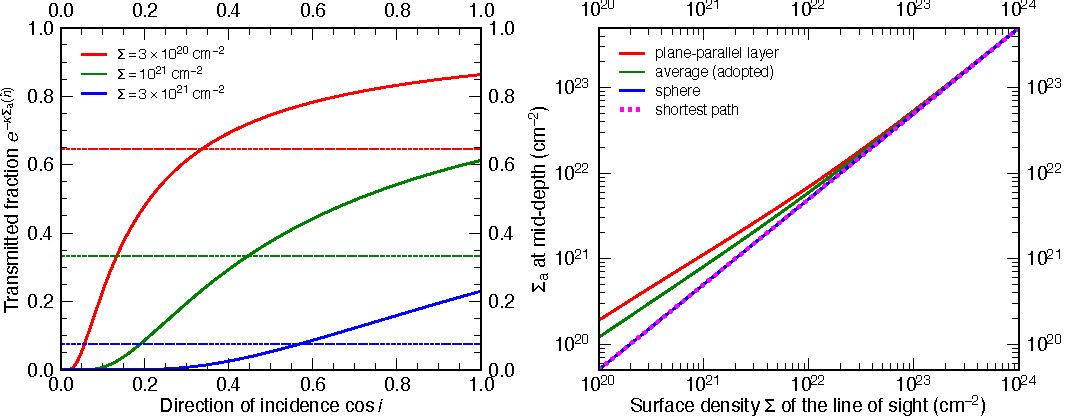
\includegraphics[width=0.85\textwidth]{fig_angular.pdf}
\caption{\emph{Left}: The fraction of the heating radiation that survives the journey inward, against the direction it comes from, 
for a parcel at mid-depth of a plane-parallel layer of three total surface densities. Plotted against the cosine of the angle, the
angular mean of each curve is the area beneath it, drawn dashed; the single column that would produce that same mean intensity is
the effective attenuating column of Eq.~(\ref{eq:seff}). \emph{Right}: that column against the total surface density of the line of
sight, for the two limiting shapes and for the average of them that is adopted, with the shortest path for comparison.}
\label{fig:angular}
\end{figure*}

We make two assumptions here. First, the opacity at the heating wavelengths is taken to be gray, with $A_{\rm V} =
N({\rm H_2})/0.94\times10^{21}$\,cm$^{-2}$ and $\tau = A_{\rm V}/1.086$. In reality, the opacity varies across the ultraviolet and
optical, so Eq.~(\ref{eq:seff}) is an average over wavelength as well as over direction. Second, the radiation field outside the
cloud is isotropic, as in the models of Sect.~\ref{sec:models}.

\subsection{The models}
\label{sec:models}

The relation between $\Sigma_{\rm a}$ and $T$ is not a free choice. It follows from radiative transfer, once the dust properties
and the radiation field are fixed. We computed a grid of models with \emph{radmc-3d} \citep{Dullemond+2012}. Each model is a
Bonnor--Ebert sphere \citep{Ebert1955, Bonnor1956} embedded in a uniform spherical cloud. It is heated from outside by the
interstellar radiation field, of strength $G_0 = 10$ in units of the local field, which includes the cosmic microwave background.
The dust opacity is that of \citet{Ossenkopf+Henning1994}, scaled to the power law $\kappa_\nu = \kappa_0(\nu/\nu_0)^2$ with
$\kappa_0 = 10.0$\,cm$^2$\,g$^{-1}$ (of dust) at $\nu_0 = 1000$\,GHz. The dust-to-gas mass ratio is $10^{-2}$ and $\muH = 2.8$.
The main grid contains 2089 models. They span the surface density of the embedding cloud, the size of the core, and its
central-to-edge density ratio (Appendix~\ref{sec:grid}). Three models reach the highest surface densities and are optically thick
in the far infrared. The correction assumes optically thin emission, so we leave these three models out. The relation is fitted to
the other 2086 models and to the models of filaments described below.

Filaments are not spheres, so we also computed models of filaments. Each one is a cylinder with the density profile $\rho(R) =
\rho_{\rm c}\,[1 + (R/R_{\rm f})^2]^{-p/2}$, truncated at the radius $R_{\rm out} = 0.5$\,pc. The flat radius $R_{\rm f}$ is
set by the half-maximum width $H$ of the surface density profile. The cylinders are computed with the same dust and the same
radiation field as the spheres, on an axisymmetric grid with a length of 7.2\,pc. We use only their middle part, where the
temperature depends on $R$ alone. We computed eight cylinders. Six of them have $p = 1.75$, $H = 40{\arcsec}$, and surface densities
on the axis of $3{\times}10^{21}$, $10^{22}$, $3{\times}10^{22}$, $5{\times}10^{22}$, $10^{23}$ and $2{\times}10^{23}$\,cm$^{-2}$.
The other two have $3{\times}10^{22}$\,cm$^{-2}$ on the axis, with $p = 2$ or with $H = 80{\arcsec}$. The cylinder with
$2{\times}10^{23}$\,cm$^{-2}$ has an optical depth of 0.84 at 100{\um} through its axis, like the three spheres that we left out,
so we leave it out as well. For each cylinder, $\Sigma_{\rm a}$ is computed from Eq.~(\ref{eq:seff}) for an infinite cylinder with
the same profile. The spheres and the cylinders are given equal total weights in the fit.

The density structure of every model is known. The attenuating column of a shell can therefore be computed along any direction by
integrating the density along that ray. Equation~(\ref{eq:seff}) is then evaluated by summing over directions. Each shell is
weighted by its mass. Near the centers of the densest cores, few photon packets of the Monte Carlo calculation arrive, and the
temperatures of the innermost cells scatter widely. We reject a shell among the ten innermost ones if its temperature differs by
more than 10\% from the median of its five neighbors. We also reject every shell inside it. The rejected shells are 1.8\% of all
shells, and they contain a negligible fraction of the mass. The fit does not depend on this choice.

\subsection{The relation}
\label{sec:relation}

The 102\,464 shells of the 2086 spheres and the 315 radii of the seven cylinders follow a single relation
(Fig.~\ref{fig:shielding}). We fit it with the function
\begin{equation}
T(\Sigma_{\rm a}) = T_{\rm f} + (T_0 - T_{\rm f}) \left(1 + \frac{\Sigma_{\rm a}}{\Sigma_\star}\right)^{-\gamma},
\label{eq:law}
\end{equation}
where $T_{\rm f} = 6.8124$\,K, $T_0 = 22.6261$\,K, $\Sigma_\star = 2.5386\times10^{21}$\,cm$^{-2}$ and $\gamma = 1.6065$. The
mass-weighted scatter about the relation is 5.2\%. The two limits have simple meanings. $T_0$ is the temperature of dust that the
radiation reaches without attenuation. $T_{\rm f}$ is the temperature that dust approaches when the radiation cannot reach it at
all; the dust is then warmed only by the little radiation that penetrates and by the microwave background. The spheres are on
average 3\% warmer than the relation, and the cylinders 2 to 3.5\% colder. A filament is thus slightly colder than a sphere at the
same $\Sigma_{\rm a}$. Leaving out any one cylinder changes the correction factor by less than 1.5\%, except for the cylinder with
$10^{23}$\,cm$^{-2}$ on the axis, which changes it by up to 4.5\% at the highest surface densities. Above
$\Sigma_{\rm a} = 10^{23}$\,cm$^{-2}$, the models contain too little mass to constrain the relation.

\begin{figure}
\centering
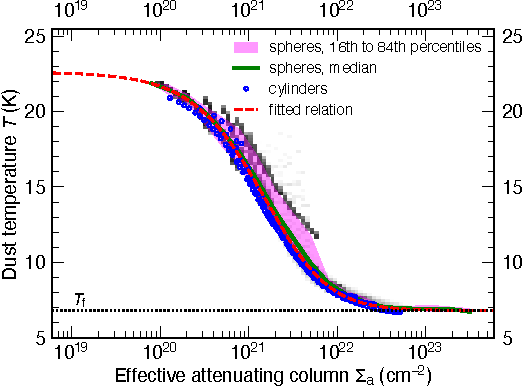
\includegraphics[width=0.9\columnwidth]{fig_shielding.pdf}
\caption{The dust temperature against the effective attenuating column $\Sigma_{\rm a}$ in the radiative transfer models. The gray
scale is the mass-weighted density of the 102\,464 shells of the 2086 spheres. The solid line and the band are their weighted
median and their 16th to 84th percentiles in bins of 0.2\,dex. The circles are the 315 radii of the seven cylinders. The dashed line
is the relation of Eq.~(\ref{eq:law}), fitted to the spheres and the cylinders with equal weights. The dotted line marks the
temperature $T_{\rm f}$ that fully shielded dust approaches.}
\label{fig:shielding}
\end{figure}

A single relation describes models that differ greatly from one another. This is the result that makes the method possible. The
size of a core and its concentration do not appear in Eq.~(\ref{eq:law}), and they do not need to. They affect the temperature only
by changing the amount of material between the dust and the radiation. The scatter about the relation, 5.2\%, measures how much
structures of different shapes differ at the same $\Sigma_{\rm a}$. It is physical, and it would not decrease with more models.

% =====================================================================

\section{The correction}
\label{sec:corr}

\begin{figure*}
\centering
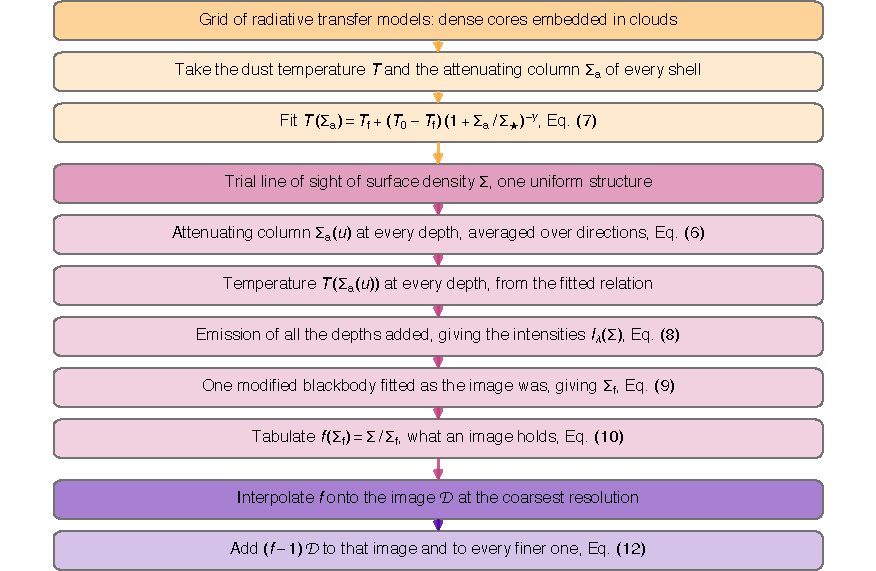
\includegraphics[width=0.75\textwidth]{fig_method.pdf}
\caption{The method step by step. The first group is the calibration, which is done once and yields the temperature relation of
Eq.~(\ref{eq:law}). The second is the calculation of Sect.~\ref{sec:factor}, repeated for every trial surface density, which
yields the table of the correction factor against the surface density that an observed image actually holds. The third is what is
then done to a reconstruction.}
\label{fig:method}
\end{figure*}

\subsection{The calculation}
\label{sec:factor}

We now have everything we need, and nothing is left to adjust. For a line of sight with the true surface density $\Sig$, the
factor is computed in five steps. (\emph{i}) We take a structure of uniform density with the total surface density $\Sig$ and
compute $\Sigma_{\rm a}$ at each depth from Eq.~(\ref{eq:seff}). (\emph{ii}) The temperature at each depth follows from
Eq.~(\ref{eq:law}). (\emph{iii}) The emergent intensity is the sum of the emission of all layers,
\begin{equation}
   \Iim_\lambda(\Sig) = \kappa_\lambda\,\eta_{\rm dg}\,\muH\,\mH\,\Sig
   \int_0^1 B_\lambda \big(T(\Sigma_{\rm a}(u))\big)\,{\rm d}u ;
\label{eq:emission}
\end{equation}
(\emph{iv}) We fit a single modified blackbody to these intensities, in the same wavebands and with the same weights as the
reconstruction. The fit gives a temperature $\Teff$ and the surface density that the reconstruction would report,
\begin{equation}
   \Sig_{\rm f}(\Sig) = \frac{\Iim_{\rm ref}(\Sig)} {\kappa_{\rm ref}\,\eta_{\rm dg}\,\muH\,\mH\,B_{\rm ref}(\Teff)} ;
\label{eq:fitted}
\end{equation}
(\emph{v}) The correction factor is the ratio of the two surface densities. It is tabulated against $\Sig_{\rm f}$, because an
observed image contains $\Sig_{\rm f}$ and not $\Sig$:
\begin{equation}
   f(\Sig_{\rm f}) = {\Sig}/{\Sig_{\rm f}} .
\label{eq:factor}
\end{equation}
Figure~\ref{fig:method} shows the five steps together with the steps before and after them.

\begin{figure}
\centering
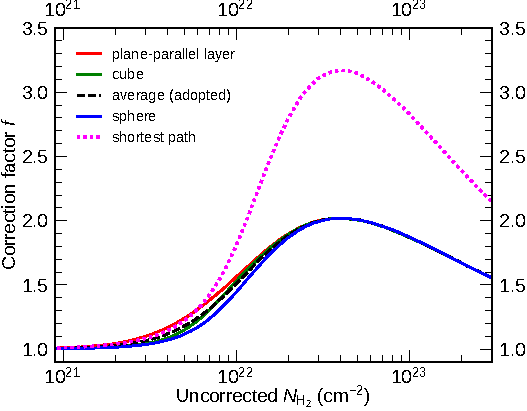
\includegraphics[width=0.85\columnwidth]{fig_relation.pdf}
\caption{The correction factor against the surface density of the uncorrected image, for a uniform plane-parallel layer, for a cube, 
for a uniform sphere, and for the average of the two that is adopted.}
\label{fig:relation}
\end{figure}

Figure~\ref{fig:relation} shows the result. The factor is unity below $10^{21}$\,cm$^{-2}$, where nothing is attenuated. It rises
steeply through the range of surface densities of most of a molecular cloud. It flattens above $10^{23}$\,cm$^{-2}$, where the
dust has reached the temperature floor and further shielding cannot cool it.

The lower panel of Fig.~\ref{fig:geometry} shows the quantity that drives the calculation, the profile of $\Sigma_{\rm a}$ along a
line of sight. At $10^{21}$\,cm$^{-2}$ the profile is nearly flat. The line of sight is then nearly isothermal, and there is almost
nothing to correct. As the surface density rises, the profile steepens and approaches the dotted line of the shortest path. Once
the material is optically thick, the oblique directions deliver nothing, and only the normal direction matters.


\subsection{Why the shape hardly matters}
\label{sec:orient}

The calculation needs a shape, but an observed field does not provide one. Cores are embedded in filaments. Filaments are curved
and blended with their neighbors. Everything lies on a background that fluctuates on all scales. It is therefore important that the
result should not depend much on the assumed shape. It does not.

Figure~\ref{fig:relation} gives the factor for a uniform sphere, a uniform cube and a uniform plane-parallel layer of the same
observed surface density. The three agree to within 10\% everywhere. Outside a narrow range near $10^{22}$\,cm$^{-2}$, they agree to
within 4\%. Figure~\ref{fig:geometry} shows why. At low surface densities nothing is attenuated, and every shape gives $f = 1$. At
high surface densities the deepest material is optically thick in every direction, and the distribution of path lengths no longer
matters. The shape matters only in between, where the correction itself is modest. In short, where the geometry would matter, the
correction is small, and where the correction is large, the geometry does not matter. We adopt the average of the sphere and the
layer, and we take their difference as the uncertainty due to the geometry.

Appendix~\ref{app:shape} explains why the sphere and the layer are the two limits. It also explains why the angular average cannot
be replaced by the column along the shortest path.

One assumption remains: each structure is taken to have a uniform density. This assumption matters much less than it seems. For a
plane-parallel line of sight it does not matter at all. A parcel of dust is shielded by the column between the parcel and the
surface. This column does not depend on how the material within it is distributed. Putting half of the material into a dense clump
does not change the amount of material. The mass of a line of sight per unit column is also constant for any density profile,
because the column is the integral of the density. Let $\Sig(s)$ be the column in front of a parcel at the depth $s$. The emission of
Eq.~(\ref{eq:emission}) integrated along the line of sight is then
\begin{equation}
   \int_0^L B_\lambda\big(T(\Sigma_{\rm a}(\Sig(s)))\big)\,\rho(s)\,{\rm d}s
   = \int_0^{\Sig} B_\lambda\big(T(\Sigma_{\rm a}(\Sig'))\big)\,{\rm d}\Sig' ,
\label{eq:invariance}
\end{equation}
and the density has disappeared. Two lines of sight with the same total surface density emit the same spectrum. It does not matter
whether their material is smooth or clumped, or whether a clump lies at the near side, in the middle, or at the far side.
Appendix~\ref{app:arrange} confirms this numerically for density profiles that differ by a factor of thirty. They reproduce the
smooth case to two parts in $10^{4}$.

Concentration and arrangement can therefore act only through the one thing that Eq.~(\ref{eq:invariance}) assumes: that the
radiation escapes along the line of sight and not across it. Their effect is modest. A sphere with a central-to-edge density ratio
of 10 needs a correction 2 to 4\% larger than a uniform sphere of the same central surface density. For a ratio of $10^3$, it needs 9
to 20\% more, and the difference grows with the surface density. A cirrus with a denser structure embedded in it is a different case.
The correction for such a line of sight is between 13\% too small and 25\% too large, depending on the depth of the structure in the
cirrus. Both effects are measured in Appendix~\ref{app:arrange}, and they enter the uncertainties of Sect.~\ref{sec:limits}.

\subsection{How it is applied}
\label{sec:apply}

The correction of an observed field needs one image of the reconstruction, the base image at some resolution $\theta_{\rm b}$:
\begin{equation}
\Sc(\theta_i) = \Sim(\theta_i) + \big[f\big(\Sim(\theta_{\rm b})\big) - 1\big]\,\Sim(\theta_{\rm b}) .
\label{eq:correction}
\end{equation}
The term in brackets is computed once and added to the image at every resolution $\theta_i$. Equation~(\ref{eq:cumulative}) allows
this, because the increments do not depend on the base image. When the base is the image being corrected ($\theta_{\rm b} =
\theta_i$), Eq.~(\ref{eq:correction}) reduces to multiplying that image by $f$. We adopt the finest image, $\theta_{\rm b} =
13.5{\arcsec}$, as the base. The factor was calibrated for the surface density that a single modified blackbody fit returns at the
resolution of the longest waveband. The finest image is sharper than any such fit, so this choice must be justified by the tests
of Sect.~\ref{sec:valid}. On the radiative transfer models, the finest base gives the most accurate masses and profiles, and it
also gives the sharpest corrected images. The base at $36.3{\arcsec}$ gives nearly the same masses and remains a conservative
alternative (Sect.~\ref{sec:base}). The correction must be applied only once. Both of our implementations mark their output and
refuse an input that has already been corrected.

\subsection{What the correction needs, and what it does not}
\label{sec:needs}

Nothing in Eqs.~(\ref{eq:seff}) to (\ref{eq:factor}) refers to the multi-resolution reconstruction. The factor is a function of one
number: the surface density that a single modified blackbody fit returns at the resolution of the longest waveband. This number can
be obtained from the observed images alone. The base image of \emph{hires} is exactly this fit. We verified this on the grid: a
modified blackbody fitted to the same wavebands with the same weights reproduces the base image of \emph{hires} to better than 1\%
for every model. The correction therefore applies to a conventional surface density map, made in the usual way from the
\emph{Herschel} intensities convolved to a common beam. Equation~(\ref{eq:correction}) then reduces to multiplying that map by
$f$.

What the reconstruction adds, and what no correction can replace, are the increments. They contain the information on scales finer
than the beam of the longest waveband. Without them, there is nothing to correct at $13.5{\arcsec}$, and the corrected map is a map at
$36.3{\arcsec}$.

The order of the operations matters when an image is decomposed into components. A parcel is shielded by the whole column along
its line of sight. The factor must therefore be evaluated on the total surface density, not on a component of it. If the image is
corrected first and the background is subtracted afterwards, the crest of a filament above its background is recovered to 2\%. If
the background is subtracted first and the remaining structure is corrected, only 73\% of the crest is recovered, because the factor
is then evaluated at a surface density that the material does not have. For the same reason, the correction must never be applied
to an image that is already corrected, or to a true surface density. Applied to the true image of the simulated sky, it would
multiply the crest of a filament by a further factor of 2.16.

One condition applies when the correction is used outside \emph{hires}. The table of $f$ is built for a particular set of wavebands
and a particular weighting of them, because $\Sig_{\rm f}$ depends on both. The table must be rebuilt if a map was made from other
wavebands or with other weights. The table cannot be replaced by anything derived from the photometry itself, for the reason given
in Appendix~\ref{app:colors}. The signature of the temperature mixing is smaller than the calibration uncertainties, so the
correction must come from models.

Two more properties follow from the construction. First, the correction is insensitive to noise, because it evaluates a smooth
function of an image and fits nothing. We added Gaussian noise of 1.5, 0.50, 0.30 and 0.15\,MJy\,sr$^{-1}$ at 160, 250, 350 and
500{\um} to the models. The total corrected surface density changed by less than 0.5\%. Second, the correction depends on the
calibration of the reference waveband only, in direct proportion, because the base image is proportional to that intensity. The
amplification by 7 to 9 found in Appendix~\ref{app:colors} does not apply here, because the colors are not used.

% =====================================================================


\section{Validation}
\label{sec:valid}

A correction can be tested only where the true surface density is known. We test it in two settings that complement each other.
The radiative transfer models are exact, but each model contains a single core in a smooth cloud. The simulated sky of
Sect.~\ref{sec:sim} contains cores, filaments and a diffuse cirrus along the same lines of sight. However, the temperatures of its
cirrus and filaments are computed analytically, not by radiative transfer. The simulated sky therefore cannot reveal an error in
Eq.~(\ref{eq:law}).

\subsection{On the radiative transfer models}
\label{sec:valgrid}

The relation of Eq.~(\ref{eq:law}) was fitted to the models of the main grid. To test the correction on models that were not used
in the fit, we computed a second grid of 1815 models. Their parameters lie between those of the main grid, and they have the same
radiation field $G_0 = 10$ (Appendix~\ref{sec:grid}). For each model, we convolved the emission to the beams of the four
wavebands and reconstructed it with \emph{hires}, as for an observation. We then corrected the reconstruction with the base image
at $13.5{\arcsec}$ and, for comparison, at $36.3{\arcsec}$. We compared the corrected images with the true surface density of the
model at the same resolution in three ways. Table~\ref{tab:valgrid} gives the results.

The first measure is the total surface density within the footprint of the model, divided by the same total in the true image.
The footprint is the area where the model stands above its surroundings in the true image at $13.5{\arcsec}$. This measure shows
whether the correction restores the right amount of material. The second measure is the mass $M$ of the core. It is the same
total with the background subtracted, divided by the same quantity in the true image. The background is the median surface density
in a ring $15{\arcsec}$ wide just outside the footprint. The third measure is the radial profile of the relative residual. The
residual is the corrected minus the true surface density, divided by the true surface density, as a function of the distance from
the center of the core. Each measure is computed for every model. Table~\ref{tab:valgrid} gives the median over the models and the
16th and 84th percentiles, which enclose the central 68\% of the models.

\begin{table}
\caption{Validation on 1815 radiative transfer models that were not used to fit the relation of Eq.~(\ref{eq:law}). Total:
the surface density summed over the footprint of the model, divided by the true value. Core mass: the same sum less the
background, divided by the same measurement on the true image. Center and $21{\arcsec}$: the relative residual of the surface
density at 3 and $21{\arcsec}$ from the center of the core. The first two columns give the median over the models, with the 16th
and 84th percentiles in parentheses; the last two give medians.}
\label{tab:valgrid}
\centering
\begin{tabular}{lcccc}
\hline\hline
\noalign{\smallskip}
\!\!\! Image & \!\!\!\! Total & \!\!\!\! Core mass & \!\!\!\!\! Center & $21{\arcsec}$\!\!\\
\noalign{\smallskip}
\hline
\noalign{\smallskip}
\!\!\! uncorr.              & \!\!\!\!\! 0.78 (0.56--0.93) & \!\!\!\!\! 0.63 (0.46--0.86) & \!\!\!\!\!\!\! $-0.44$ & \!\!\!\!\!\!\! $-0.21$\!\!\\
\!\!\! base $36.3{\arcsec}$ & \!\!\!\!\! 0.99 (0.91--1.02) & \!\!\!\!\! 0.94 (0.71--1.13) & \!\!\!\!\!\!\! $-0.13$ & \!\!\!\!\!\!\! $+0.02$\!\!\\
\!\!\! base $13.5{\arcsec}$ & \!\!\!\!\! 0.99 (0.92--1.03) & \!\!\!\!\! 0.98 (0.76--1.17) & \!\!\!\!\!\!\! $-0.09$ & \!\!\!\!\!\!\! $+0.03$\!\!\\
\noalign{\smallskip}
\hline
\end{tabular}
\end{table}

\begin{figure*}
\centering
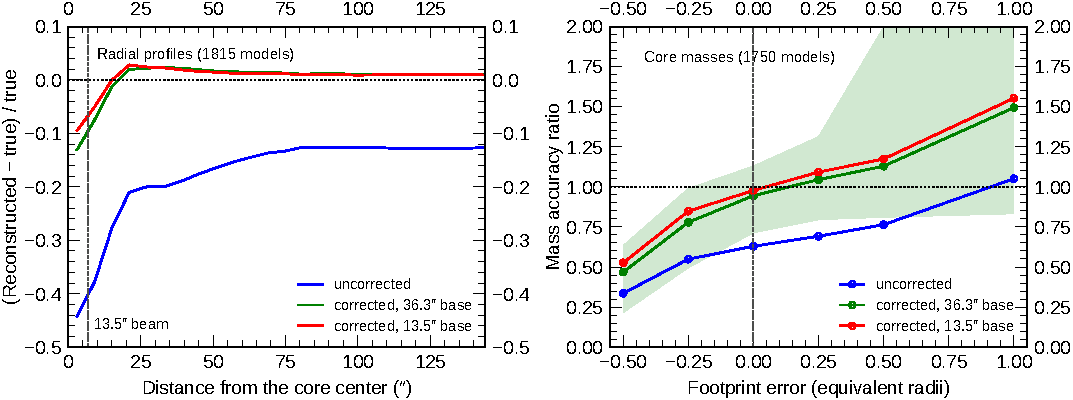
\includegraphics[width=0.9\textwidth]{fig_grid_validation.pdf}
\caption{The correction tested on 1815 radiative transfer models that were not used to fit the relation of
Eq.~(\ref{eq:law}). \emph{Left}: the relative residual of the surface density, the reconstructed minus the true value divided by
the true value, against the distance from the center of the core, as the median over the models. The dashed line marks half the
beam of $13.5{\arcsec}$. \emph{Right}: the mass of the core, divided by the true mass, when the footprint within which it is
measured is too small (negative abscissa) or too large (positive abscissa) by the given fraction of its equivalent radius. The
background is always taken in a ring just outside the footprint used. The lines are medians over the models, and the band marks
the 16th to 84th percentiles for the correction with the base at $36.3{\arcsec}$.}
\label{fig:valgrid}
\end{figure*}

Without the correction, the reconstruction contains 78\% of the true surface density and 63\% of the core mass. The deficit is
largest at the center of the core, where it reaches 44\%. The correction restores the total to 99\% and the core mass to 98\% in the
median. Beyond $15{\arcsec}$ from the center, the residual is within 3\% (Fig.~\ref{fig:valgrid}, left). A deficit of 9\%
remains at the center of the core, at $3{\arcsec}$. No correction that depends on the surface density alone can remove it. The
center of a core is colder than the center of a uniform structure with the same surface density, and the surface density does not
reveal this. The base at $36.3{\arcsec}$ gives almost the same totals but a larger deficit at the center. The factor it applies
varies more slowly across the core than the core itself (Sect.~\ref{sec:base}).

The spread over the models is larger than these medians. For one core in six, the corrected mass is more than 24\% too low. For
another one in six, it is more than 17\% too high. A correction that depends on the surface density alone cannot remove this
spread. Models with the same surface density can differ in how their temperature varies along the line of sight.

\paragraph{The footprint matters more than the correction.}
In a real image, the footprint of a core is not known. It must be estimated, together with the background beneath the core. The
right panel of Fig.~\ref{fig:valgrid} shows how an error in the footprint changes the measured mass. A footprint that is too small
by a quarter of its radius lowers the median corrected mass from 0.98 to 0.85 of the true mass. A footprint that is too small by
half its radius lowers it to 0.53, because part of the core is then counted as background. A footprint that is too large by a quarter
or a half of its radius raises the median mass to 1.09 or 1.17, and the spread over the models widens sharply. These errors are
lower limits. The models lie in a cloud of uniform density, whose surface density declines smoothly with radius. A real core is
surrounded by filaments and other cores. They enter the background ring in ways that no model reproduces.

The correction removes a systematic deficit of about 40\% in the masses of cores. What remains, a few percent in the median, is
smaller than the error caused by a plausible misjudgment of the footprint and the background. We return to this in
Sect.~\ref{sec:limits}.

\subsection{On a simulated sky}
\label{sec:sim}

The models of Sect.~\ref{sec:valgrid} are single spheres, but an observed field is not. We therefore built a simulated sky, in
which the true surface density is known by construction. It contains a diffuse cirrus, seven filaments and 96 embedded cores. The
cirrus is plane-parallel. The filaments are cylinders with the profile observed in real clouds, with $H = 40{\arcsec}$ and wings
falling as $r^{-0.75}$. The temperatures of the cirrus and of the filaments are computed from Eq.~(\ref{eq:law}). The cores are
radiative transfer models of the grid, with known masses. We computed the intensities at 70 to 500{\um}, convolved them to the
corresponding beams, sampled them on $3{\arcsec}$ pixels, and passed them through \emph{hires} as for an observation. In a second
version of the sky, the filaments are inclined at random to the plane of the sky.

The simulated sky tests what the models cannot: the superposition of several structures along a line of sight. It has a limitation
of its own, however. A pixel that contains several structures is warmer than a single body with the same total surface density. A
correction that assumes a single body over-corrects such a pixel (Appendix~\ref{app:arrange}). The simulated sky therefore measures
this bias together with the accuracy of the correction.

\begin{table}
\caption{Fraction of the true value recovered on the simulated sky at $13.5{\arcsec}$, before the correction and after it with the
base image at $13.5{\arcsec}$ (the adopted one) and at $36.3{\arcsec}$, for filaments in the plane of the sky and inclined at
random. Total: the surface density summed over the field. Core center: the central pixel of each core. Core mass: the surface
density within one Bonnor--Ebert radius less the background measured between 2 and 2.5 radii, divided by the same measurement on
the true image. The core entries are medians over the cores.}
\label{tab:sim}
\centering
\begin{tabular}{llccc}
\hline\hline
\noalign{\smallskip}
Sky & Quantity & Uncorr. & Base $13.5{\arcsec}$ & Base $36.3{\arcsec}$ \\
\noalign{\smallskip}
\hline
\noalign{\smallskip}
plane    & total       & 0.776 & 1.133 & 1.106 \\
         & core center & 0.542 & 1.064 & 1.010 \\
         & core mass   & 0.566 & 1.096 & 1.006 \\
inclined & total       & 0.788 & 1.160 & 1.133 \\
         & core center & 0.553 & 1.064 & 1.010 \\
         & core mass   & 0.561 & 1.088 & 1.008 \\
\noalign{\smallskip}
\hline
\end{tabular}
\end{table}

\begin{figure*}
\centering
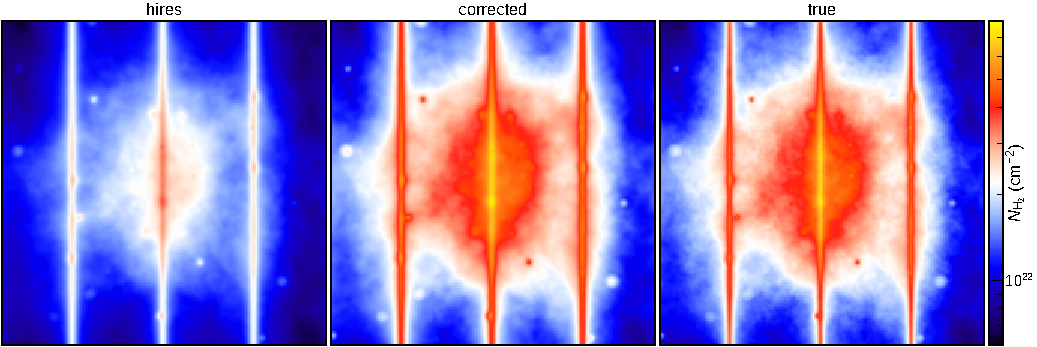
\includegraphics[width=\textwidth]{fig_simsky.pdf}
\caption{A part of the simulated sky at $13.5{\arcsec}$: the reconstruction of \emph{hires}, the same image after the correction
of Eq.~(\ref{eq:correction}), and the true surface density. The three panels share one logarithmic scale.}
\label{fig:simsky}
\end{figure*}

\begin{figure}
\centering
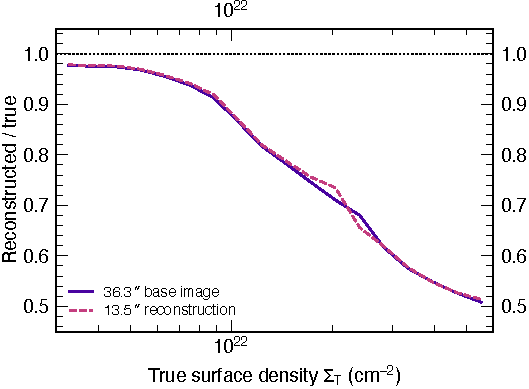
\includegraphics[width=0.9\columnwidth]{fig_deficit.pdf}
\caption{The reconstruction of the simulated sky divided by its true surface density, in bins of the true surface density, at the
coarsest resolution and at the finest. The two curves lie almost on top of one another: the increments that the reconstruction
adds between those resolutions are very nearly right, and the deficit is the same fraction of the surface density at both
resolutions.}
\label{fig:deficit}
\end{figure}

Figure~\ref{fig:simsky} shows the sky before and after the correction, together with the truth. Table~\ref{tab:sim} gives the
numbers. Before the correction, the reconstruction contains 78\% of the true surface density, 54\% of it at the centers of the cores,
and 57\% of the core masses. After the correction, the core masses are 9 to 10\% too high with the adopted base and within 1\% with
the base at $36.3{\arcsec}$. The total surface density is 13 to 16\% too high with either base. This excess is the superposition
bias described above. Most of the area of the field is diffuse, and its cirrus and filaments shield each other less than the single
body that the correction assumes. The cores of the sky lie on this over-corrected background. On the models, where each core lies in
its own smooth cloud, the same correction gives masses 2\% too low (Sect.~\ref{sec:valgrid}). The two tests therefore bracket the
truth. Neither offset is large compared with the error due to the background (Sect.~\ref{sec:valgrid}). Figure~\ref{fig:deficit}
shows on the simulated sky the property found in Sect.~\ref{sec:deficit} on the models. At every surface density, the
reconstruction falls below the truth by the same fraction at both resolutions. The factor can therefore be evaluated at either
resolution.

\subsection{Where the correction fails}
\label{sec:fails}

\begin{figure*}
\centering
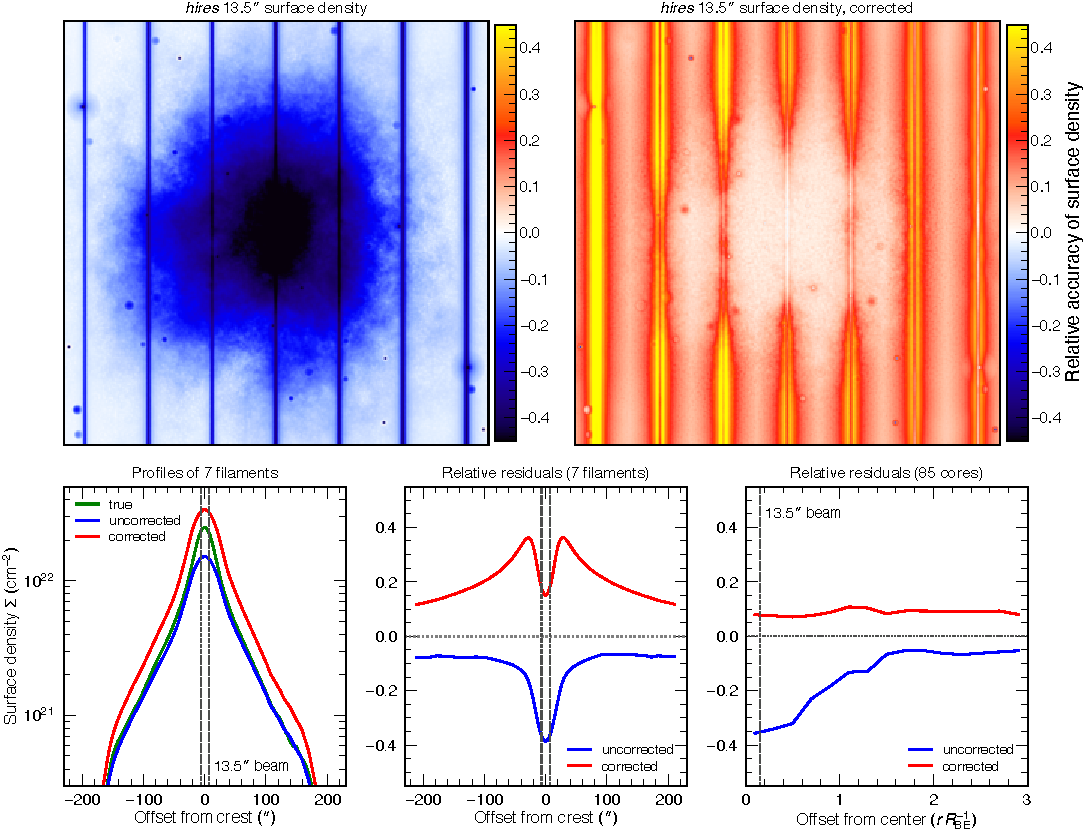
\includegraphics[width=\textwidth]{fig_simsky4_residual.pdf}
\caption{\emph{Upper panels}: the relative residual of the reconstruction at $13.5{\arcsec}$ against the true surface density of
the simulated sky, before and after the correction, on the same scale. \emph{Lower panels}: the profiles themselves, stacked over
the seven filaments and with their backgrounds removed; the same profiles as relative residuals; and the residual stacked over the
injected cores against the radius in units of the Bonnor--Ebert radius. The dashed lines mark the $13.5{\arcsec}$ beam.}
\label{fig:residual}
\end{figure*}

The numbers of Table~\ref{tab:sim} are averages. Figure~\ref{fig:residual} shows the variations behind them. Before the correction,
the reconstruction is too low everywhere: by about 10\% over the diffuse field and by 40\% at the centers of the cores and on the
crests of the filaments. After the correction, the crests of the filaments are within 6 to 12\% of the truth. However, the flanks of
the filaments are over-corrected by up to 30\% at about $20{\arcsec}$ from the crest, and a weaker ring of over-correction
surrounds the cores.

These over-corrected flanks are an artifact of the simulated sky, not of the correction. The simulated sky shields each parcel of a
filament by the column along the radius, from the parcel outward. A parcel on the flank of a real filament also receives radiation
along directions that cross the dense axis, and these directions shield it strongly. The flanks of the simulated filaments are
therefore too warm, and their deficit is too small. We verified this with an analytic calculation for the filament profile of the
sky, without cirrus and without a beam. With the angle-averaged shielding of Eq.~(\ref{eq:seff}), the corrected profile is below the
truth everywhere, by 11\% on the crest and by less than 2\% beyond $24{\arcsec}$. With the radial shielding of the simulated sky, the
crest is 20\% too low and the flanks are 3 to 5\% too high. In the simulated sky, the superposition with the cirrus and the beam add
to this over-correction. \draftnote{Radiative transfer models of filaments will replace the simulated filaments in this test.}

The correction of the crests of filaments and of the centers of cores is limited in the same way as on the models. A correction
that depends on the surface density alone cannot distinguish a given surface density on the axis of a concentrated structure from
the same surface density in a uniform structure. We tested corrections that use the fitted temperature as a second observable,
calibrated on the radiative transfer models. They fail for an instructive reason, described in Appendix~\ref{app:tcorr}. The effect
of the correction on the widths $H$, the slopes and the linear densities $\Lambda$ of the simulated filaments is given in
Appendix~\ref{app:filaments}.

\subsection{The choice of the base image}
\label{sec:base}

Nothing in Sect.~\ref{sec:corr} ties the correction to one resolution. Figure~\ref{fig:base} in Appendix~\ref{app:filaments} shows
what the choice of the base image changes. A finer base gives a correction that follows the structures more closely. The width $H$ of
a filament decreases from 78 to $72{\arcsec}$, and the index of its wings rises from 0.73 to 0.75, against the true values of
$50{\arcsec}$ and 0.82. On the simulated sky, a finer base raises the core masses by about 9\%. On the radiative transfer models, it
raises them by 3\%, which brings them closer to the truth (Table~\ref{tab:valgrid}). The two bases differ by less than the error due
to the background. We adopt the finest base, which gives the sharper images. The base at $36.3{\arcsec}$ remains a conservative
alternative. It is useful when a corrected map at the resolution of the longest waveband is needed, because it then reduces to
multiplying a conventional surface density map by $f$.

% =====================================================================

\section{Application to the Aquila cloud}
\label{sec:aquila}

We applied the correction to a $31\arcmin \times 31\arcmin$ field of the Aquila cloud. The field was observed with \emph{Herschel}
at 70, 160, 250, 350 and 500{\um} \citep{Andre+2010, Konyves+2015}. We adopt a distance of 260\,pc. The factor is evaluated on the
reconstruction at $13.5{\arcsec}$ and applied to it. The field contains 375\,769 pixels of $3{\arcsec}$.

The median correction factor over the field is 1.49, and the largest factor is 2.02. The factor is below 1.11, 1.35, 1.74 and 2.02
for 1, 25, 75 and 99\% of the pixels. The correction is therefore significant everywhere in the field. The total surface density of
the field increases by a factor of 1.68.

The distribution of surface densities changes more than the median factor suggests, because the factor rises with the surface
density. The median surface density of the field increases from $9.7{\times}10^{21}$ to $1.5{\times}10^{22}$\,cm$^{-2}$, and its
99th percentile from $5.6{\times}10^{22}$ to $1.1{\times}10^{23}$\,cm$^{-2}$. The number of pixels above $10^{22}$\,cm$^{-2}$
increases from 178\,641 to 288\,069. Above $3{\times}10^{22}$\,cm$^{-2}$ it increases from 17\,041 to 71\,479, and above
$10^{23}$\,cm$^{-2}$ from 666 to 5183, a factor of eight. A much larger part of the cloud therefore exceeds any given threshold
after the correction. This matters for any criterion based on a surface density threshold, such as a threshold for star formation.
The dust temperature that follows from the corrected surface density has a median of 12.8\,K over the field.
It is below 9.4 and 19.5\,K for 1 and 99\% of the pixels.

\begin{figure*}
\centering
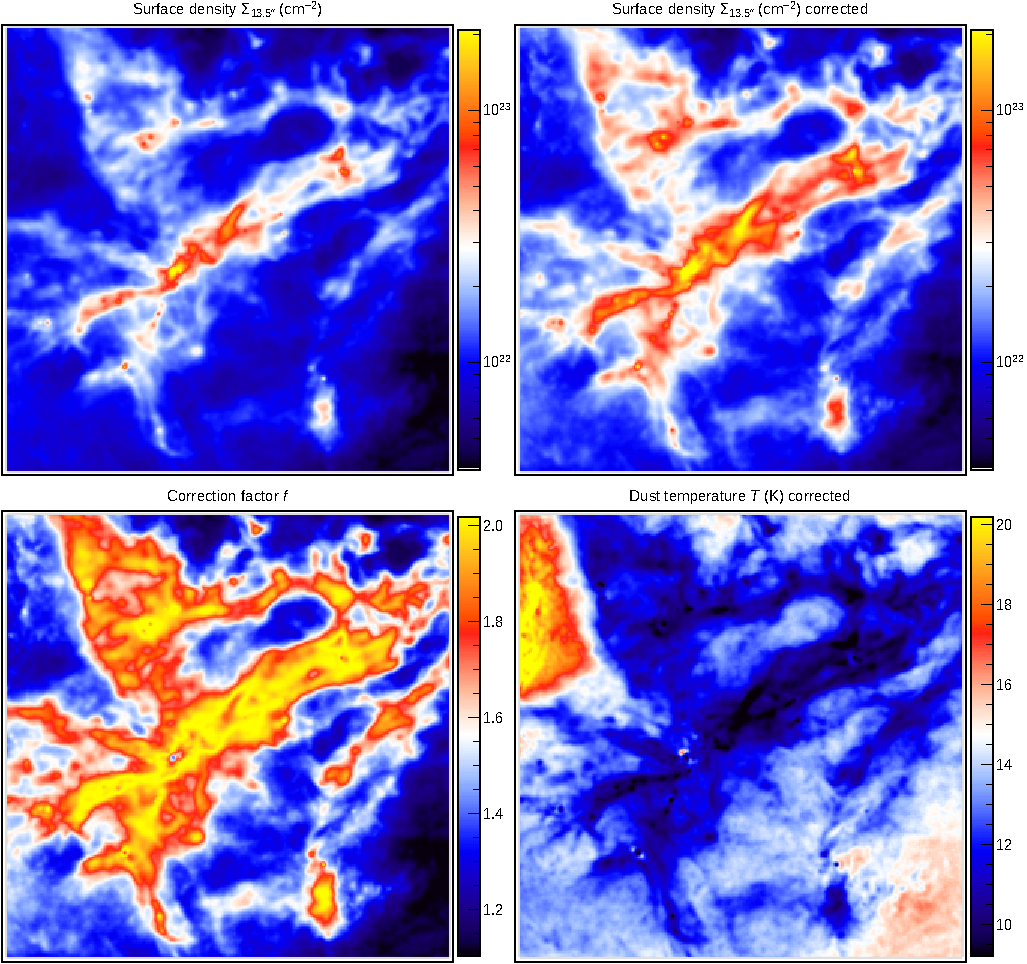
\includegraphics[width=\textwidth]{fig_aquila.pdf}
\caption{The Aquila field at $13.5{\arcsec}$. \emph{Upper panels}: the surface density before and after the correction, on a
common logarithmic scale. \emph{Lower panels}: the correction factor $f$ and the dust temperature that follows from the corrected
surface density. The factor is smallest in the diffuse material and largest along the crests of the filaments and at the cores.}
\label{fig:aquila}
\end{figure*}

Figure~\ref{fig:aquila} shows the field before and after the correction, together with $f$ and the dust temperature. The correction
is not a uniform rescaling. The factor is smallest in the diffuse material between the structures and largest along the crests of
the filaments and at the cores. The correction therefore raises the contrast of the image as well as its overall level. In some
places, the dust of Aquila is heated by a field stronger than $G_0 = 10$. The warm corner at the upper left of the temperature map
is the clearest example. Section~\ref{sec:field} discusses the uncertainty due to the radiation field.

\section{Uncertainties and limitations}
\label{sec:limits}

The first term below concerns the measurement of a source, not the correction itself. It is the largest term for the masses of
cores, which are the main application of the correction. The other terms are uncertainties of the correction.

\subsection{The background and the footprint}
\label{sec:bgerr}

The mass of a core is the surface density within its footprint minus the background beneath it. Neither the footprint nor the
background is known in a real image. Section~\ref{sec:valgrid} measured the effect on models with the simplest possible
background. A footprint that is wrong by a quarter of its radius changes the median mass by $-13$ to $+12$\%. A footprint that is
wrong by half its radius changes it by $-46$ to $+20$\%. For footprints that are too large, the spread over the models widens
sharply. In a real cloud, a core lies on filaments and among other cores. The background beneath it is not a smooth continuation of
its surroundings \citep{Menshchikov2016}, and the errors are larger. They are discussed in Sect.~3.4.7 of
\citet{Menshchikov2021method} and in Sect.~4.4 of \citet{Menshchikov2023}. The correction does not change any of this, because it
acts on the image, not on the source. This is the largest uncertainty of a core mass. It is also the reason why we preferred the
simplest correction to the more complex ones of Appendix~\ref{app:tcorr}. None of them changed the median core mass by more than a
few percent, which is much less than this term.

\subsection{The radiation field}
\label{sec:field}

The relation of Eq.~(\ref{eq:law}), and therefore $f$, was calibrated for $G_0 = 10$. To measure the effect of a different field, we
computed the models of the grid for nine fields from $G_0 = 0.98$ to 483, in steps of a factor of 2.17 (Appendix~\ref{app:field}).
We compared the factor required by each set of models with the factor that the correction applies, at surface densities from
$4{\times}10^{21}$ to $2.5{\times}10^{23}$\,cm$^{-2}$ (Table~\ref{tab:field}). In fields with $G_0 \approx 1$ to 2, the applied
factor is too large, and the corrected surface density is too high by up to 33\%. At $G_0 = 10$ itself, the error is within 4\% up
to $6{\times}10^{22}$\,cm$^{-2}$ and $-13$\% above. In fields of a few tens, the correction is too small by up to 20\%. Above
$G_0 \approx 200$, it is again too large at the highest surface densities. Most nearby star-forming clouds are heated by fields within a factor of a few of $G_0 = 10$. For a cloud in a much
weaker or much stronger field, the correction should be calibrated again on models computed for that field. We also examined
whether the field could be derived from the observed dust temperature, pixel by pixel. It cannot. A pixel can be warmer than the
relation predicts for two reasons. It may be heated by a stronger field, and then it needs more correction. Or it may lie on the
flank of a structure or behind a warm cirrus, and then it needs less correction (Appendix~\ref{app:tcorr}).

\subsection{The arrangement along the line of sight}

An observed line of sight contains several structures at unknown depths. The method replaces them by a single uniform body with the
same total surface density. Equation~(\ref{eq:invariance}) shows that this replacement is exact in the plane-parallel limit. The
error is therefore caused only by the radiation that escapes across the line of sight. Appendix~\ref{app:arrange} measures this
error in two forms. First, a concentrated structure needs more correction than a uniform one: 2 to 4\% more for a central-to-edge
density ratio of 10 and 9 to 20\% more for a ratio of $10^3$. Second, for a structure embedded in a cirrus, the corrected surface density
is between 13\% too low and 25\% too high, depending on the depth of the structure in the cirrus. The largest over-correction, 25\%,
occurs when a dense cirrus lies entirely behind or entirely in front of the structure. A weak cirrus leaves the structure nearly
isolated, and the correction is then too small by 8 to 13\% at any depth. The depth of a structure within a cloud cannot be observed. This uncertainty therefore cannot be reduced by a
better calculation. Section~\ref{sec:fails} shows how it appears in an image: as a pattern that follows the structures, not as a
uniform offset.

\subsection{The temperature relation and its floor}

The size of the correction depends on Eq.~(\ref{eq:law}), and in particular on the temperature $T_{\rm f} = 6.8$\,K that dust
approaches when it is completely shielded. The factor is very sensitive to $T_{\rm f}$. Lowering $T_{\rm f}$ by 1\,K raises the
factor by 35\% at $10^{22}$\,cm$^{-2}$ and by 59\% at $3{\times}10^{22}$\,cm$^{-2}$. Raising $T_{\rm f}$ by 1\,K lowers the factor by
14 and 24\%, respectively. The floor is therefore the part of the relation that most needs to be right. The fit to 2086 spheres and
seven cylinders constrains it well, and the temperatures of the densest models approach $T_{\rm f}$ smoothly
(Fig.~\ref{fig:shielding}). Fitted to only 15 spheres, as in an earlier stage of this work, the relation gave $T_{\rm f} = 6.2$\,K
and much larger factors at high surface densities. Above $10^{23}$\,cm$^{-2}$, the models contain too little mass to constrain the
relation. Observations of prestellar cores usually give central temperatures of 7 to 9\,K. An analytic relation in common use
places the floor at 10\,K. A floor that high would substantially lower the factor at the highest surface densities.

\subsection{The geometry}

The calculation needs a shape, and an observed field does not provide one. Figure~\ref{fig:relation} shows that this hardly
matters. A uniform sphere and a uniform layer of the same surface density need factors within 8\% of each other everywhere, and
within 4\% outside a narrow range near $10^{22}$\,cm$^{-2}$. We average the two and take half of their difference as the
uncertainty. It is 4\% at most.

\subsection{What the correction does not do}

The correction acts on an image, not on a source. The subtraction of the background of a core and the definition of its footprint
are left to the method that extracts the source. The correction also assumes that the dust is heated from outside, as in the
models. A line of sight through a protostar contains an internal source, and its temperature gradient is reversed.
Equation~(\ref{eq:correction}) does not apply there. Such positions should be identified by their compact 70{\um} emission and left
uncorrected.

\section{Conclusions}
\label{sec:conclusions}

Surface density images of molecular clouds are derived by fitting one modified blackbody to each pixel. These images are
systematically too low wherever the dust temperature varies along the line of sight. The deficit reaches a factor of three in the
densest material.

The deficit cannot be measured from the observed colors. Its signature in the spectrum is 1 to 6\% of the intensities, while the
deficit itself is 9 to 38\%. A method that derived one from the other would amplify the photometric errors 7 to 9 times. This is far
beyond the accuracy of \emph{Herschel} photometry. The correction must therefore come from radiative transfer.

Radiative transfer provides a single relation between the dust temperature and the effective column $\Sigma_{\rm a}$ that shields
the dust. It describes 2086 models of embedded Bonnor--Ebert spheres and seven models of filaments, with a scatter of 5.2\%. The size and the
concentration of a structure enter only through $\Sigma_{\rm a}$, which is an average over all directions of the incoming radiation.
As a result, a sphere, a cube and a plane-parallel layer of the same surface density need factors within 10\% of each other. The
relation gives the correction factor $f$ as an explicit function of the observed surface density, with no fitted parameters.

The correction applies to an image. It applies to a conventional surface density map at the resolution of the longest waveband and
to every image of a multi-resolution reconstruction. In a reconstruction, the deficit is the same fraction of the surface density at
every resolution. We evaluate the factor on the finest image, which gives the sharpest corrected images and, on the radiative
transfer models, the most accurate masses.

We tested the correction on 1815 radiative transfer models that were not used in the calibration. It raises the median core mass
from 0.63 to 0.98 of the true mass and the total surface density from 0.78 to 0.99. Beyond $15{\arcsec}$ from the center of a core,
the corrected profile is within 3\% of the truth. A deficit of 9\% remains at the center. On a simulated sky of cirrus, filaments
and embedded cores, the core masses are 9\% too high, because the diffuse background beneath them is over-corrected.

The correction leaves only a few percent in the median core mass. This is less than the error caused by a plausible misjudgment of
the footprint and the background of a core: $-13$ to $+12$\% for a footprint wrong by a quarter of its radius, even for the simplest
models. A correction that depends on the surface density alone is therefore sufficient. Corrections that also use the fitted
temperature are not worth their complexity, because a warm pixel may be heated by a stronger field or may lie on the flank of a
structure, and the two cases need opposite corrections.

The correction is calibrated for $G_0 = 10$. Models computed for $G_0 = 1$ to 500 show that it is accurate to about 20\% for
$G_0 = 5$ to 100, and that it is too large by up to a third in the weakest fields. Its other uncertainties are the floor temperature
$T_{\rm f}$ of fully shielded dust, to which $f$ is very sensitive above $10^{22}$\,cm$^{-2}$, and the arrangement of the material
along the line of sight. The latter changes the corrected surface density by $-13$ to $+25$\%, and it cannot be reduced, because the
depth of a structure within a cloud cannot be observed. Applied to a field of the Aquila cloud, the correction raises the total
surface density by a factor of 1.68 and the number of pixels above $10^{23}$\,cm$^{-2}$ eightfold.

\begin{acknowledgements}
\draftnote{To be written.}
\end{acknowledgements}

\bibliographystyle{aa}
\bibliography{hires2_correction}

% =====================================================================

\appendix
\nolinenumbers 

\section{The grids of models}
\label{sec:grid}

All models are Bonnor--Ebert spheres embedded in a uniform spherical cloud. They are heated from outside by the interstellar
radiation field and computed with \emph{radmc-3d} for the dust of Sect.~\ref{sec:models}. We used three grids, which are summarized
in Table~\ref{tab:grids}.

The main grid varies three parameters. The first is the surface density $\Sig_{\rm emb}$ of the embedding cloud, in steps of a
factor of two from $3.75\times10^{20}$ to $9.6\times10^{22}$\,cm$^{-2}$. The second is the half-maximum size of the Bonnor--Ebert
sphere, from 0.02 to 0.25\,pc. The third is its central-to-edge density ratio, from nearly uniform ($\rho_{\rm c}/\rho_{\rm e}
\approx 1.2$) to strongly concentrated ($\sim 10^3$). \draftnote{Please check these ranges and the numbers of steps along each
axis.} Three more models extend the grid to $\Sig_{\rm emb}$ of $1.9$ to $7.9\times10^{23}$\,cm$^{-2}$. They are optically thick in
the far infrared and are not used in the calibration (Sect.~\ref{sec:models}). The temperature of each model, tabulated shell by
shell, enters the relation of Eq.~(\ref{eq:law}).

The models of the subdivision grid lie between the models of the main grid. They test the correction on models that were not used
in the relation. For each model, the intensities at 70 to 500{\um} were convolved to the beams of the wavebands, reconstructed by
\emph{hires} and corrected. The true surface density was convolved to the same resolutions. The footprint of a model is the area of
the convolved true image that stands above the embedding cloud.

The grid of radiation fields repeats 305 models of the main grid, together with 34 models at a tenth embedding surface density of
$1.92\times10^{23}$\,cm$^{-2}$. They are computed for nine strengths of the radiation field, from $G_0 = 0.98$ to 483, in steps of
a factor of 2.17. The lowest field is the weakest that our implementation of the radiation field allows. About five models per
field were not computed, because they required the largest images. They do not affect the results of Appendix~\ref{app:field}.

\begin{table}
\caption{The grids of radiative transfer models.}
\label{tab:grids}
\centering
\begin{tabular}{lccl}
\hline\hline
\noalign{\smallskip}
Grid & $G_0$ & Models & Used for \\
\noalign{\smallskip}
\hline
\noalign{\smallskip}
Main          & 10           & 2089          & the relation of Eq.~(\ref{eq:law}) \\
Subdivision   & 10           & 1815          & validation, Sect.~\ref{sec:valgrid} \\
Radiation fields & 0.98--483 & $9\times339$ & Appendix~\ref{app:field} \\
\noalign{\smallskip}
\hline
\end{tabular}
\end{table}

\section{The arrangement of the material along the line of sight}
\label{app:arrange}

The correction is applied pixel by pixel. A pixel receives the emission of everything along its line of sight, and a single modified
blackbody is fitted to this sum. The fit is therefore biased by the whole distribution of dust temperatures along the line of sight,
not by the temperature of any one structure. The method replaces this distribution by the one of a single uniform body with the
same total surface density. This appendix measures the error of this replacement.

\subsection{The invariance}
\label{app:invariance}

In a plane-parallel geometry, the emergent emission depends only on the total surface density. The attenuating column of a parcel
is set by the column between the parcel and each surface. This column does not depend on how the material is distributed. The mass
of a line of sight per unit column is constant for any density profile. This is Eq.~(\ref{eq:invariance}). To check the algebra
and the integrations, we computed the four intensities of a line of sight of $2{\times}10^{22}$\,cm$^{-2}$ that contains a clump
thirty times denser than its surroundings. We placed the clump at 15, 50 and 85\% of the depth. The intensities differ from those of
the smooth line of sight by at most $2.1{\times}10^{-4}$, $4.6{\times}10^{-5}$ and $1.2{\times}10^{-4}$, which is the accuracy of
the numerical integration. Neither the concentration of the material nor the position of the clump has any effect.

\subsection{Concentration}
\label{app:concentr}

In the plane-parallel limit, the density profile has no effect at all. Concentration can therefore act only through the radiation
that escapes across the line of sight. A bounded structure allows this escape, and a layer does not. We measure the effect on a
sphere with the density $\rho(r) \propto (1 + r^2/a^2)^{-1}$ out to its boundary. The sphere is normalized so that the column
through its center equals the observed one, and $a$ is set by the central-to-edge density ratio. The parcels along the central line
of sight are weighted by their density, as in the emission. For each parcel, the column is integrated along the ray to the
boundary in every direction of the average.

\begin{table}
\caption{Correction factor required by the central line of sight of a sphere of the given central surface density, for four
central-to-edge density ratios. The first column is a uniform sphere.}
\label{tab:concentr}
\centering
\begin{tabular}{lcccc}
\hline\hline
\noalign{\smallskip}
$\Sig$ (cm$^{-2}$) & uniform & $10$ & $10^2$ & $10^3$ \\
\noalign{\smallskip}
\hline
\noalign{\smallskip}
$5{\times}10^{21}$ & 1.093 & 1.132 & 1.167 & 1.186 \\
$1{\times}10^{22}$ & 1.289 & 1.345 & 1.420 & 1.468 \\
$3{\times}10^{22}$ & 1.781 & 1.838 & 1.980 & 2.129 \\
$1{\times}10^{23}$ & 2.005 & 2.054 & 2.168 & 2.378 \\
\noalign{\smallskip}
\hline
\end{tabular}
\end{table}

Table~\ref{tab:concentr} gives the result. Concentration always raises the required correction, because the mass of a concentrated
structure lies where the shielding is deepest. The effect is 2 to 4\% for a density ratio of 10 and 9 to 20\% for a ratio of $10^3$.
It is one-sided. A correction built on uniform structures therefore underestimates the deficit of a concentrated structure and never
overestimates it.

\subsection{Two superposed components}
\label{app:twocomp}

The second case is a line of sight that crosses a diffuse cirrus with a denser structure embedded in it at an unknown depth. We take
a plane-parallel cirrus of surface density $\Sig_{\rm c}$. The material at the column depth $x$ in the cirrus is shielded by the
angular average of $x/|\mu|$ toward the observer and of $(\Sig_{\rm c} - x)/|\mu|$ away from the observer. A uniform sphere with the
surface density $\Sig_{\rm s}$ through its center is embedded in the cirrus. A fraction $q$ of the cirrus lies in front of the
sphere. A parcel at the signed position $z$ along the diameter of the sphere, in units of its radius, is shielded by its own sphere
over the path
\begin{equation}
   l(z,\psi) = -z\cos\psi + \sqrt{1 - z^2\sin^2\psi} ,
\label{eq:lsphere}
\end{equation}
in units of the radius. It is also shielded by the cirrus over $q\,\Sig_{\rm c}/|\cos\psi|$ toward the observer and
$(1-q)\,\Sig_{\rm c}/|\cos\psi|$ away from the observer. The sign of $z$ must be kept. With $|z|$ instead, the sphere would be
symmetric about its center regardless of the cirrus in front of it, and the result would be wrong for every $q$ except one half. We
take the angular average of Eq.~(\ref{eq:seff}) over $\psi$ with the isotropic weight $\sin\psi$. The temperature of every parcel
follows from Eq.~(\ref{eq:law}). The emission of the cirrus and of the sphere are added with their masses, and one modified
blackbody is fitted to the sum, exactly as in the reconstruction. This gives the fitted surface density $\Sig_{\rm f}$ of the
composite line of sight and the factor $\Sig/\Sig_{\rm f}$ that it requires. The method sees only $\Sig_{\rm f}$ and applies
$f(\Sig_{\rm f})$ of Eq.~(\ref{eq:factor}). The error of the corrected surface density is therefore $f(\Sig_{\rm f})\,\Sig_{\rm
f}/\Sig - 1$. The construction is symmetric under $q \rightarrow 1-q$, as it must be, and so are the computed factors.

\begin{figure*}
\centering
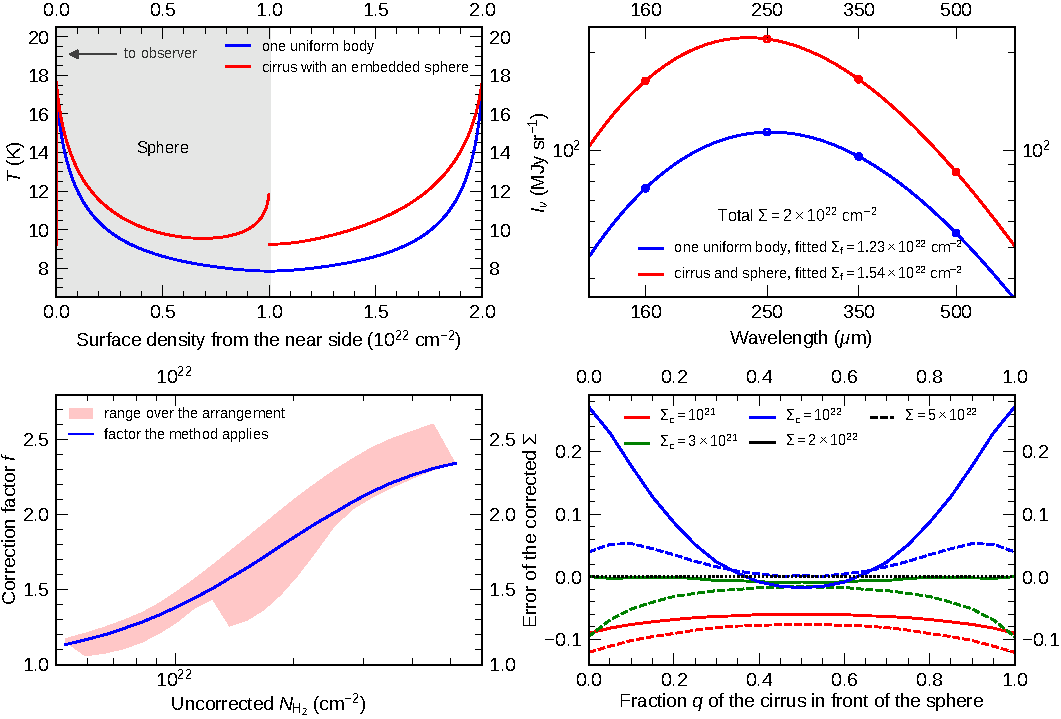
\includegraphics[width=0.9\textwidth]{fig_superposition.pdf}
\caption{Superposition of a cirrus and a sphere. \emph{Upper left}: The dust temperature along a line of sight of
$2{\times}10^{22}$\,cm$^{-2}$. One curve is for the uniform body that the method assumes. The other curve is for the same surface
density divided equally between a cirrus and a uniform sphere at the near side of the cirrus ($q = 0$). \emph{Upper right}: The
emission of the two lines of sight, with the surface density $\Sig_{\rm f}$ that a single modified blackbody fit returns. The two
lines of sight have the same true surface density. \emph{Lower left}: The factor that the method applies and the range of factors
that the composite lines of sight require, both against the observed (fitted) surface density. The range covers cirrus surface
densities $\Sig_{\rm c}$ of $10^{21}$, $3{\times}10^{21}$ and $10^{22}$\,cm$^{-2}$ and all positions of the sphere. \emph{Lower
right}: The error of the corrected surface density against the fraction $q$ of the cirrus in front of the sphere.}
\label{fig:superposition}
\end{figure*}

Figure~\ref{fig:superposition} gives the result. The error of the corrected surface density ranges from $-13$ to $+25$\%. Its sign
depends on the cirrus. A weak cirrus ($\Sig_{\rm c} = 10^{21}$\,cm$^{-2}$) leaves the sphere nearly isolated. The sphere needs more
correction than the average of a sphere and a layer, so the correction is too small by 8 to 13\%, at any depth. A dense cirrus
($\Sig_{\rm c} = 10^{22}$\,cm$^{-2}$) with the sphere at one of its sides makes the line of sight warmer than a single body. The
correction is then too large, by up to 25\%. When the sphere lies near the middle of a dense cirrus, the error is only a few
percent. The error is symmetric about $q = 0.5$, as it must be.

The upper panels of Fig.~\ref{fig:superposition} show why the effect exists. The two lines of sight have exactly the same total
surface density. In one of them, half of the surface density is a sphere at the near side of the cirrus. The sphere loses radiation
sideways, and nothing in front of it blocks the incoming radiation. This line of sight is warmer and brighter in all four
wavebands. A single modified blackbody fit returns $1.44{\times}10^{22}$\,cm$^{-2}$ for it and $1.23{\times}10^{22}$\,cm$^{-2}$ for the
uniform body. The composite line of sight requires a factor of 1.39, but the method sees $1.44{\times}10^{22}$\,cm$^{-2}$ and applies
the factor that a uniform body with this observed surface density requires, which is 1.72. The corrected surface density is then
24\% too high.

Nothing observable distinguishes the two lines of sight. The depth of a structure within a cloud cannot be measured, and no better
calculation can recover it. The error of $-13$ to $+25$\% (Sect.~\ref{sec:limits}) is therefore an irreducible uncertainty of any
method of this kind, not a defect of this one.

\section{Why the observed colors cannot supply the correction}
\label{app:colors}
\label{sec:amplification}

One could try to measure the temperature structure directly, by fitting more than one component to the observed spectrum of each
line of sight. Without noise, this works. A free two-temperature fit from 160 to 500{\um} recovers 0.96 to 1.00 of the true surface
density at the centers of the four models, against 0.62 to 0.91 for the single-temperature fit. With noise, it does not work.
Table~\ref{tab:signature} shows why.

\begin{table}
\caption{Signature of the temperature mixing in the four-band spectral energy distribution at the center of each model, compared
with the deficit it produces. Columns two to five give the relative residuals, in percent, of the best single-component fit to the
noiseless intensities; column six their root-mean-square; column seven the fraction of the true surface density that the
single-component fit recovers.}
\label{tab:signature}
\centering
\begin{tabular}{lcccccc}
\hline\hline
\noalign{\smallskip}
$\rho_{\rm c}/\rho_{\rm e}$ & 160 & 250 & 350 & 500 & rms & recovered \\
\noalign{\smallskip}
\hline
\noalign{\smallskip}
1.18  & $+0.92$ & $-1.37$ & $-0.44$ & $+0.93$ & 0.97 & 0.914 \\
1.28  & $+0.88$ & $-2.16$ & $-0.46$ & $+1.82$ & 1.50 & 0.869 \\
4.47  & $+3.46$ & $-6.44$ & $-1.56$ & $+5.39$ & 4.61 & 0.680 \\
90.8  & $+3.76$ & $-8.04$ & $-1.64$ & $+7.27$ & 5.79 & 0.619 \\
\noalign{\smallskip}
\hline
\end{tabular}
\end{table}

The residuals have the same pattern for every model: positive at 160 and 500{\um} and negative at 250 and 350{\um}. This is the
broadening of the spectrum by a mixture of temperatures. The deficit divided by the root-mean-square residual is 8.9, 8.7, 6.9 and
6.6. Any method that infers the deficit from the colors therefore amplifies the relative photometric errors by a factor of 7 to 9.
The calibration uncertainties of \emph{Herschel} observations of Aquila are 20\% at 70 to 160{\um} and 10\% at 250 to 500{\um}
\citep{Konyves+2015}. For the two weakly concentrated models, the whole signature is below the photometric accuracy. A test that
accepts a second component only where it significantly improves the fit never accepts it, for any pixel of any model.

\begin{figure*}
\centering
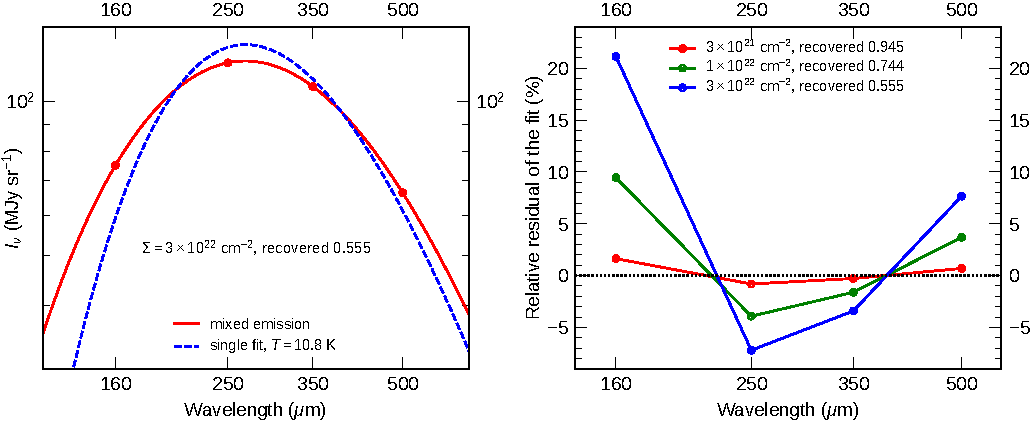
\includegraphics[width=0.9\textwidth]{fig_mixing.pdf}
\caption{\emph{Left}: the emission of a line of sight of $3{\times}10^{22}$\,cm$^{-2}$, the sum over depth of material at every
temperature, with the single modified blackbody fitted to it in the four wavebands and with the weights that the reconstruction
uses. The fit is drawn toward the warmer and brighter material, so the temperature it returns is too high and the surface density
that follows from it is too low. \emph{Right}: the relative residuals of that fit, waveband by waveband, for three total surface densities,
with the fraction of the true surface density recovered beside each. The pattern is always the same, positive at the ends and
negative in the middle, and it grows with the surface density, but it never rises above the calibration uncertainties of 20{\%} at
160{\um} and 10{\%} at the three longer wavebands.}
\label{fig:mixing}
\end{figure*}

Figure~\ref{fig:mixing} shows the emission of a mixed line of sight, the single modified blackbody fitted to it, and the remaining
residuals. The correction must therefore be calibrated on models in which the answer is known.

\section{The radiation field}
\label{app:field}

The relation of Eq.~(\ref{eq:law}) was measured for a single field, $G_0 = 10$. A stronger field heats the dust at every
attenuating column, and this changes the deficit of the fit. To measure the effect, we tested the correction on the grid of
radiation fields of Appendix~\ref{sec:grid}. For each field, every pixel of every model was reconstructed and assigned to a bin of
fitted surface density. In each bin, we took the median over the pixels of the factor that restores the true surface density.
Table~\ref{tab:field} compares this factor with the factor that the correction applies. It gives the relative error of the corrected
surface density, which is the applied factor divided by the required factor, minus one.

\begin{table}
\caption{Relative error of the corrected surface density, in percent, for models computed in radiation fields of strength $G_0$,
in four ranges of the uncorrected surface density $\Sig$ (in cm$^{-2}$). Positive values mean that the correction is too large.
The values are medians over the pixels of all models of each field, weighted by the number of pixels.}
\label{tab:field}
\centering
\begin{tabular}{rcccc}
\hline\hline
\noalign{\smallskip}
$G_0$ & $\log\Sig$: 21.6--22.0 & 22.0--22.4 & 22.4--22.8 & 22.8--23.4 \\
\noalign{\smallskip}
\hline
\noalign{\smallskip}
0.98 & $+13$ & $+33$ & $+29$ & $+15$ \\
2.12 & $+14$ & $+28$ & $+24$ & $+10$ \\
4.61 & $+6$  & $+16$ & $+14$ & $-3$  \\
10   & $+1$  & $+4$  & $-1$  & $-13$ \\
21.7 & $-7$  & $-9$  & $-7$  & $-17$ \\
47.1 & $-11$ & $-16$ & $-13$ & $-20$ \\
102  & $-13$ & $-10$ & $-7$  & $-12$ \\
222  & $-7$  & $0$   & $+6$  & $+2$  \\
483  & $-1$  & $+8$  & $+23$ & $+18$ \\
\noalign{\smallskip}
\hline
\end{tabular}
\end{table}

The error changes sign twice. The correction is too large in the weakest fields and too small in fields of a few tens. In the
strongest fields, it is again too large at the highest surface densities. The deficit of a single-temperature fit depends on how the
temperature varies along the line of sight, not on the temperature itself. A stronger field changes this variation differently at
different depths. No simple rescaling of Eq.~(\ref{eq:law}) with the field can therefore reproduce the table. At $G_0 = 10$, the
models of this grid reproduce the correction to 4\% below $6{\times}10^{22}$\,cm$^{-2}$. Above that, the correction is 13\% too small for
these spheres, which are slightly warmer than the relation fitted to spheres and filaments together.

For a cloud in a field very different from $G_0 = 10$, the correction needs a relation measured in that field. The procedure of
Sect.~\ref{sec:law} applies without change. The field varies over large scales. It could be estimated from the temperatures of the
diffuse material smoothed over several arcminutes, but only in a large map. In a small map, most pixels lie on structures
(Appendix~\ref{app:tcorr}).

\section{Corrections that read the fitted temperature}
\label{app:tcorr}

The reconstruction gives a dust temperature for every pixel, together with the surface density. If the temperature of a pixel
differs from the one that the relation predicts at its surface density, the temperature carries information that the surface
density does not. We tested four ways of using it, all calibrated on the radiative transfer models. None was adopted, and the reason
is the same for all four.

The first method was a table of the required factor, measured directly on the models, as a function of three observables. They are
the surface density, the fitted temperature, and the contrast between the images at $13.5{\arcsec}$ and $36.3{\arcsec}$, which
distinguishes the crest of a structure from its flank. The second method multiplied the factor of Eq.~(\ref{eq:factor}) by a smooth
function of the surface density and of the offset of the fitted temperature from the relation. This function was fitted to the
grid of radiation fields of Appendix~\ref{app:field}. On the models, it predicted the required factor to within 7\% in every field,
and to within 6\% for a field left out of the fit. The third method was a table of the factor against surface density and
temperature, computed like Eq.~(\ref{eq:factor}) from analytic lines of sight through spheres, cylinders and layers embedded in a
diffuse medium. The fourth method kept the factor of Eq.~(\ref{eq:factor}), but redistributed the correction within each beam of the
coarsest image to follow the shape of the finest image.

On the radiative transfer models of the subdivision grid, the first two methods raised the median core mass by 9 and 3\% relative to
the adopted correction, and the fourth changed it by 2\%. The third method was tested on the grid of radiation fields. In fields of
$G_0 = 20$ to 50, it under-corrected the dense material by a factor of 1.5 to 1.7. On the simulated sky, the first two methods
over-corrected the flanks of the filaments even more than the adopted correction. The first method also produced a correction
factor with visible structure on the scale of its bins. The fourth method narrowed the filaments slightly and weakened the rings
around extended cores, but not around compact ones. In the Aquila field, it copied the small-scale texture of the finest image,
including its noise, into the factor.

The reason is that a warm pixel is ambiguous. A pixel can be warmer than the relation predicts for two reasons. First, a stronger
radiation field may heat it. The radiative transfer models then say that it needs more correction. Second, it may lie on the flank of
a structure, near its surface, or its line of sight may also cross a warm cirrus. It then needs less correction. The models used for
the calibration contain only the first case, and the simulated sky mostly the second. A correction that uses the temperature is
therefore right in one case and wrong in the other. The fitted temperature of a single pixel cannot distinguish the two cases. The
radiation field varies over parsecs, and the warmth of a flank varies over the width of a filament. The field could therefore be
estimated in principle from the temperature of the diffuse material, smoothed over several arcminutes. In the Aquila field, however,
only 12\% of the pixels are diffuse enough, and most of them lie in one corner. The estimate would then be an extrapolation over most
of the field. None of these corrections changed the core mass by more than the error due to the background (Sect.~\ref{sec:bgerr}),
so we adopted the simplest one.

\section{Filaments and cores on the simulated sky}
\label{app:filaments}

\draftnote{This appendix describes the simulated filaments, whose flanks are too warm (Sect.~\ref{sec:fails}). It will be revised
with the radiative transfer models of filaments.} Table~\ref{tab:widths} gives the shape of the filaments of the simulated sky,
measured on the median profile of each filament along its length. Figure~\ref{fig:masses} gives the masses of the cores and the
linear densities $\Lambda$ of the filaments. The background beneath a filament is fitted together with its profile, as the constant
$B$ of $A\,r^{-\alpha} + B$ between $20{\arcsec}$ and $180{\arcsec}$ from the crest. The wings of these filaments fall so slowly that
no radius within the spacing of the filaments reaches the background.

\begin{table}
\caption{Shape of the filaments of the simulated sky, as the median over the seven filaments: the half-maximum width $H$ above the
fitted background, the index $\alpha$ of the wings, the linear density $\Lambda$ within $\pm100{\arcsec}$ and the amplitude of the 
crest above the background, the last two as fractions of the true values. The filaments were built with a width of $40{\arcsec}$, 
which the beam of $13.5{\arcsec}$ broadens to about $42{\arcsec}$, and wings falling as $r^{-0.75}$.}
\label{tab:widths}
\centering
\begin{tabular}{lcccc}
\hline\hline
\noalign{\smallskip}
 &\!\!\!\! True &\!\!\!\! Uncorr. &\!\!\!\! Base $13.5{\arcsec}$ &\!\!\!\! Base $36.3{\arcsec}$\\
\noalign{\smallskip}
\hline
\noalign{\smallskip}
width $H$                  &\!\!\!\! $50.0{\arcsec}$ &\!\!\!\! $93.0{\arcsec}$ &\!\!\!\! $71.8{\arcsec}$ &\!\!\!\! $78.2{\arcsec}$\\
index $\alpha$             &\!\!\!\! 0.82            &\!\!\!\! 0.57            &\!\!\!\! 0.75            &\!\!\!\! 0.73\\
linear density $\Lambda$   &\!\!\!\! 1               &\!\!\!\! 0.87            &\!\!\!\! 1.47            &\!\!\!\! 1.44\\
crest amplitude            &\!\!\!\! 1               &\!\!\!\! 0.60            &\!\!\!\! 1.20            &\!\!\!\! 1.12\\
\noalign{\smallskip}
\hline
\end{tabular}
\end{table}

\begin{figure*}
\centering
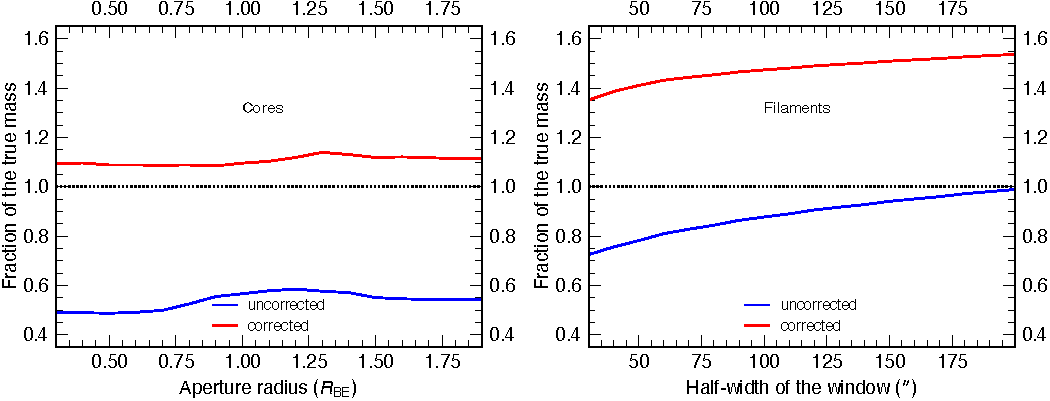
\includegraphics[width=0.9\textwidth]{fig_masses.pdf}
\caption{Masses recovered from the simulated sky, as fractions of the true values, before and after the correction with the base
at $13.5{\arcsec}$. \emph{Left}: the mass of a core, against the radius of the aperture in units of the Bonnor--Ebert radius, with
the background taken between 2 and 2.5 radii. \emph{Right}: the linear density $\Lambda$ of a filament, against the half-width of the
window over which the profile is integrated, above the fitted background. Both are medians, over the injected cores and over the
seven filaments.}
\label{fig:masses}
\end{figure*}

\begin{figure}
\centering
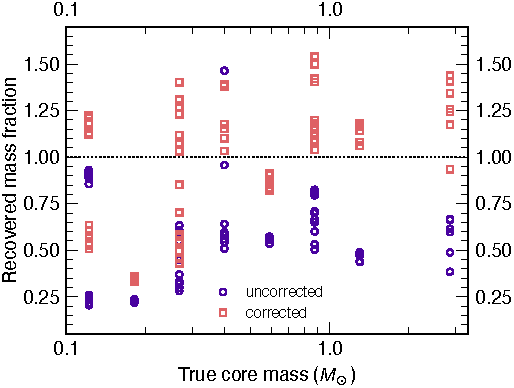
\includegraphics[width=0.9\columnwidth]{fig_core_recovery.pdf}
\caption{Integrated surface density of each injected core above its local background, as a fraction of the true value, before and
after the correction, against the true mass of the core. The dotted line marks a perfect recovery.}
\label{fig:cores}
\end{figure}

\begin{figure*}
\centering
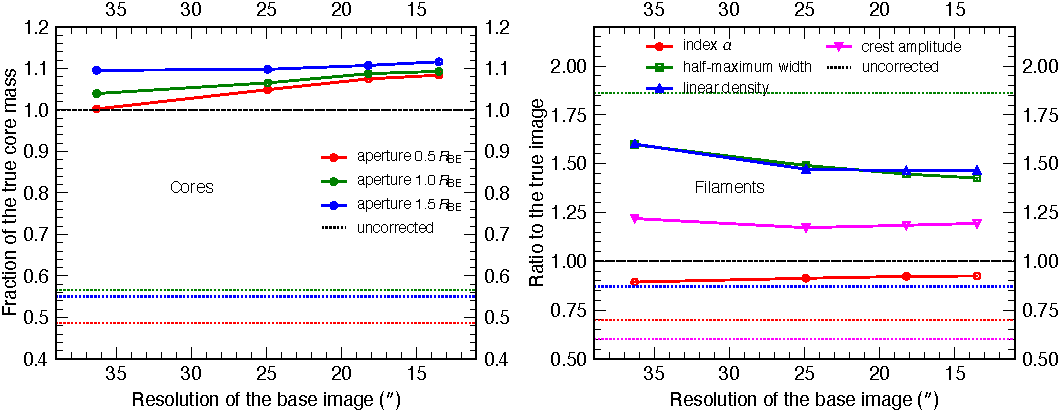
\includegraphics[width=\textwidth]{fig_base.pdf}
\caption{What the choice of the base image changes on the simulated sky. The factor is evaluated on the reconstruction at the
resolution on the abscissa and the correction is added to the image at $13.5{\arcsec}$, which is Eq.~(\ref{eq:correction}) with the
base taken in turn at each available resolution. \emph{Left}: the mass of a core recovered within three apertures, in units of the
Bonnor--Ebert radius. \emph{Right}: the shape of a filament, as ratios to the true image so that one axis serves for all four
quantities. Dotted lines mark the uncorrected reconstruction and the dashed line the true value.}
\label{fig:base}
\end{figure*}

The true image gives $\alpha = 0.82$, while the filaments were built with 0.75. The difference comes from the beam and from the
flattening of the inner profile. The uncorrected reconstruction gives 0.57, which is far too shallow, because the crest is suppressed
much more than the wings. The correction returns $\alpha$ to 0.75. The width $H$ is not restored. Without the correction, the
filaments are 86\% too wide, because the suppression of the crest flattens the profile. After the correction, they are still 44\% too
wide, because the over-corrected flanks keep the profile wide. For the same reason, $\Lambda$ is 35 to 55\% too high, depending on
the window (Fig.~\ref{fig:masses}, right). The cores are much less affected. Their masses depend little on the aperture out to one
Bonnor--Ebert radius (Fig.~\ref{fig:masses}, left). Core by core, the median recovered fraction of the mass above the background is
1.12 after the correction and 0.56 before it (Fig.~\ref{fig:cores}).

Every curve of Fig.~\ref{fig:masses} is a ratio of the reconstruction to the truth, both measured in the same way. An error of the
background that affects both images equally cancels in the ratio. The filament curves therefore show the over-correction of the
flanks, not the background. The absolute linear density of a filament is a different matter. It is uncertain for reasons that have
nothing to do with the correction. Two of them act here. The first is a near-degeneracy. A constant and a tail falling as
$r^{-0.75}$ are almost the same function over any usable range, so the fitted constant absorbs part of the filament. On these
profiles, the fitted $B$ is 0.65 to 0.80 of the true cirrus beneath the crest. The second reason is the curvature of the background.
A background that is convex over the extent of a filament lies above any straight line drawn across it. An interpolated background is
therefore too low. The error is largest beneath the filament and vanishes at the interpolation points. It adds a centrally peaked
bump to the profile, which increases the mass and steepens the measured index. On the simulated cirrus, a straight line is accurate
to better than 1\% over baselines of up to $\pm600{\arcsec}$, and it underestimates the background by 13\% at $\pm900{\arcsec}$. The
effect is negligible for a core and grows with the size of the structure. A further difficulty is that the background beneath a
structure is not a smooth continuation of its surroundings \citep{Menshchikov2016}. Removing the structure leaves an empty volume in
its place, so the background to be subtracted has the shape of a crater. These problems are discussed in Sect.~3.4.7 of
\citet{Menshchikov2021method} and in Sect.~4.4 of \citet{Menshchikov2023}. The correction does not address them, and it does not
make them worse.

A linear density $\Lambda$ obtained in this way is uncertain by tens of percent, with or without the correction. A better
$\Lambda$ requires a better treatment of the background, not a better correction.

\section{Why the sphere and the layer are the limits}
\label{app:shape}

\begin{figure*}
\centering
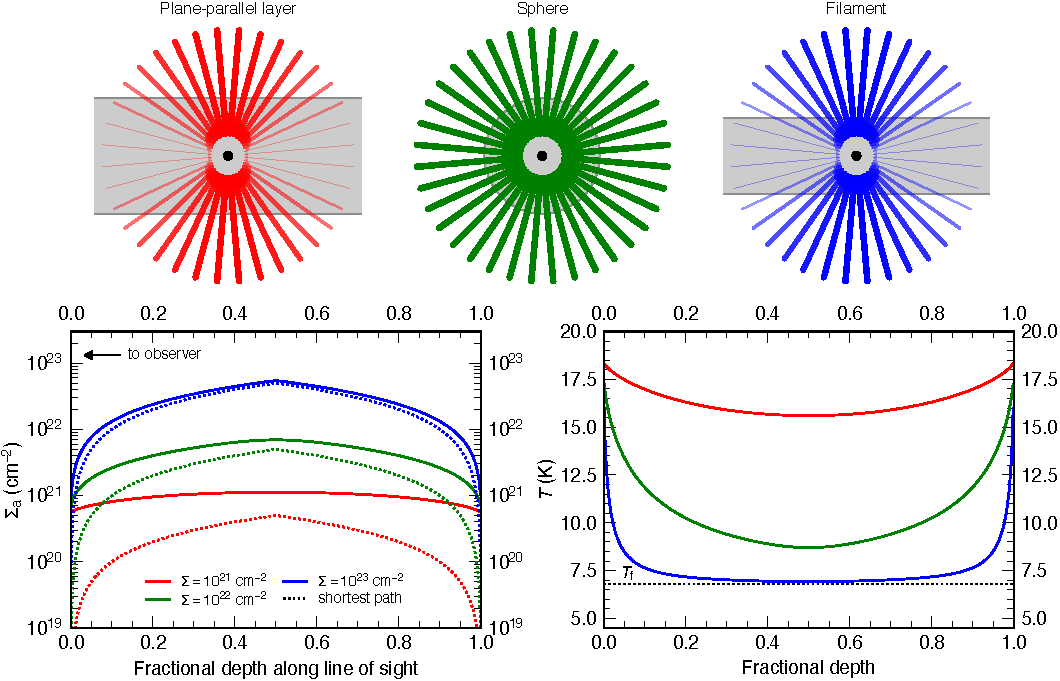
\includegraphics[width=0.8\linewidth]{fig_geometry.pdf}
\caption{\emph{Upper panels}: the radiation that heats a parcel of dust, marked by the black point, arrives from every direction
having crossed columns of very different length. The arrows are drawn thicker where less material has been crossed. In a layer
almost everything arrives along the normal; at the center of a sphere no direction is favored; a filament is intermediate, short
across and long along its axis. \emph{Lower panel}: the effective attenuating column of Eq.~(\ref{eq:seff}) along a line of sight
through a layer, as a fraction of the surface density the observer measures, for three total surface densities. The dotted line is 
what the shortest path alone would give.}
\label{fig:geometry}
\end{figure*}

The cube in Fig.~\ref{fig:relation} shows that the sphere and the layer are indeed the limits. The cube has the symmetry of neither
of them. Its factor lies between them at every surface density, within 6\% of the sphere and within 3\% of the layer. The layer is an
extreme case because it is unbounded across the line of sight. For a parcel at the mid-plane, the path to the boundary is the
half-thickness divided by the cosine of the angle to the normal. This path diverges as the angle approaches $90\degr$, so a whole
band of directions near the plane of the layer delivers no radiation, however thin the layer is. At $10^{22}$\,cm$^{-2}$, the
directions within $30\degr$ of the normal deliver 64\% of the mean intensity, and those within $45\degr$ deliver 93\%. In a
bounded body, the path is finite in every direction, and no direction is lost. The sphere is the opposite extreme: a compact body
with a given central surface density blocks less of the sky than any other body with that surface density. Every real cloud lies
between the two limits, and the range between them is the full effect of the shape. This is why the method needs no assumption
about the shape of a cloud.

The dotted curve of Fig.~\ref{fig:relation} shows what happens if the angular average is replaced by the column along the shortest
path, with the geometric factor of one quarter. A sphere, a layer and a filament share this factor when averaged over their bodies
and over isotropic orientations. Below $3{\times}10^{21}$\,cm$^{-2}$, this simpler treatment agrees with the full calculation to 1\%.
Above $10^{22}$\,cm$^{-2}$ it diverges, and at $10^{23}$\,cm$^{-2}$ it overestimates the correction by half. The shortest path gives
too little shielding to the material near the surfaces: its column falls to zero at the surface, while the oblique directions still
shield the surface material. The surface material is then too warm, the temperature contrast along the line of sight is too large,
and the deficit is overestimated. The angular average is therefore not a refinement of the shortest path. It gives a different
answer, and the models support it.

\end{document}
